\documentclass[11pt,a4paper]{article}
\usepackage[margin=2.3cm]{geometry}
\usepackage{lmodern}
\usepackage[T1]{fontenc}
\usepackage[utf8]{inputenc}
\usepackage{microtype}
\usepackage{amsmath,amssymb}
\usepackage{graphicx}
\usepackage{booktabs}
\usepackage{float}
\usepackage{xcolor}
\usepackage[font=small,labelfont=bf]{caption}
\usepackage{enumitem}
\usepackage{fancyhdr}
\usepackage{array}
\usepackage[colorlinks=true,linkcolor=blue!50!black,citecolor=blue!50!black,urlcolor=blue!50!black]{hyperref}
\graphicspath{{../results/plots/}}
\setlist{itemsep=2pt,topsep=3pt}
\emergencystretch=3em
\pagestyle{fancy}\fancyhf{}
\rhead{\small ML-based structural response prediction}\lhead{\small Technical report}\cfoot{\thepage}
\renewcommand{\headrulewidth}{0.4pt}
\newcommand{\smax}{\sigma_{\max}}
\newcommand{\dmax}{\delta_{\max}}

\begin{document}
%==================================================================== TITLE
\begin{titlepage}
\centering
\vspace*{2.5cm}
{\LARGE\bfseries Machine Learning-Based Structural Failure Prediction\\[4pt] and Stress Analysis Under Variable Mechanical Loading\par}
\vspace{1.2cm}
{\large Technical Report\par}
\vspace{0.6cm}
{\large Harshit Pala\\ B.Tech, Engineering and Computational Mechanics\\ Indian Institute of Technology Delhi\par}
\vspace{1.2cm}
{\normalsize Undergraduate research project\par}
\vfill
\begin{minipage}{0.86\textwidth}\small
\textbf{Data provenance.} All data in this report are \emph{synthetic} and were generated from closed-form
Euler--Bernoulli beam theory. No experimental measurements or finite-element simulations were used. All numerical
results were produced by the accompanying code (\texttt{run\_pipeline.py}, random seed 42) and are read
automatically from \texttt{results/experiment\_results.json} when this report is built.\\[4pt]
\textbf{Software backends used for the reported results:} <<BACKEND_SENTENCE>>
\end{minipage}
\vspace{1cm}

{\small Report generated <<DATE>>\par}
\end{titlepage}

\tableofcontents
\newpage
%==================================================================== ABSTRACT
\section*{Abstract}
\addcontentsline{toc}{section}{Abstract}
This project investigates how accurately data-driven regression and classification models can reproduce the
structural response of an end-loaded rectangular cantilever when geometry, load and material properties vary
simultaneously. A reproducible dataset of <<N>> physically valid beams was generated with Euler--Bernoulli theory,
filtered for slenderness, small deflection and a bounded stress-to-yield ratio. Three model families---a random
forest, a histogram-based gradient-boosted tree ensemble and a multi-layer perceptron (MLP)---were tuned on a
validation split and evaluated once on a held-out test split of <<NTEST>> beams. The MLP, trained on log-transformed
inputs and targets, predicted maximum bending stress with $R^2=<<MLP_S_R2>>$ (median absolute error
<<MLP_S_MED>>\,\%) and tip deflection with $R^2=<<MLP_D_R2>>$ (median error <<MLP_D_MED>>\,\%), clearly
outperforming gradient boosting ($R^2=<<GB_S_R2>>$ / <<GB_D_R2>>) and the random forest ($R^2=<<RF_S_R2>>$ /
<<RF_D_R2>>). For the yield criterion (factor of safety $<1$) the best direct classifier reached
$F_1=<<MLP_C_F1>>$, while thresholding the factor of safety implied by the MLP stress prediction reached
$F_1=<<DER_F1>>$, its only error occurring at a true factor of safety of <<DER_ERR_FOS>>. Sensitivity sweeps show that
the MLP recovers the exact power-law exponents of beam theory (e.g.\ $\partial\ln\smax/\partial\ln h=<<MLP_H_SLOPE>>$
versus $-2$), whereas tree ensembles distort trends near the edges of the data and fail to extrapolate: when trained on
forces up to <<OOD_THR>>\,N their median stress error on larger forces rose to <<OOD_RF>>\,\% (random forest) and
<<OOD_GB>>\,\% (boosting) compared with <<OOD_MLP>>\,\% for the MLP. Because the reference model is a product of powers, a
linear regression in log space reproduces it exactly; this is used as a physics-informed reference that frames the
limits of what the benchmark can show.

%==================================================================== INTRODUCTION
\section{Introduction}
Structural design repeatedly evaluates how a component responds to loads: peak stress, deformation, and the margin
against yielding. For complex geometries these quantities come from numerical solvers such as the finite element
method, whose cost becomes significant when thousands of evaluations are needed---in design-space exploration,
optimisation, uncertainty quantification or interactive tools. \emph{Surrogate models} replace the expensive solver with
a fast approximation learned from a set of solver evaluations~\cite{forrester2008}.

Before surrogates can be trusted on problems without closed-form solutions, it is instructive to study them on a
problem where the exact answer is known everywhere. The cantilever beam with an end load is such a problem: its
response follows from elementary beam theory~\cite{gere2013}, so every prediction can be checked exactly, both
inside and outside the training domain. This project uses that setting to answer three questions:
\begin{enumerate}
\item How accurately do common ML regressors approximate stress and deflection for unseen beam configurations?
\item Do the learned models reproduce the \emph{physical trends} (scaling laws) of beam theory, not just low average error?
\item How reliably can the models classify whether the yield criterion is exceeded, and where do they fail?
\end{enumerate}

\paragraph{Scope.} The project is a methodological benchmark. It does not claim novelty, and the trained models are
\emph{not} faster than the analytical formulas they imitate (Section~\ref{sec:timing}); their value lies in what they
reveal about model choice, data representation and generalisation for later work with expensive solvers.

%==================================================================== PROBLEM STATEMENT
\section{Problem statement}
Given the six parameters $\mathbf{x}=(L,b,h,F,E,\sigma_y)$ of a rectangular cantilever (length, width, thickness,
tip force, Young's modulus, yield strength), learn mappings
\begin{equation}
\mathbf{x}\;\mapsto\;\bigl(\smax,\ \dmax\bigr), \qquad \mathbf{x}\;\mapsto\;\mathbb{1}[\mathrm{FoS}<1],
\end{equation}
from examples, and derive the maximum strain $\varepsilon_{\max}$ and factor of safety FoS from the predicted stress.
Performance is measured on beams never seen during training or model selection. All quantities are in SI units.

%==================================================================== ENGINEERING BACKGROUND
\section{Engineering background}
\begin{figure}[H]\centering
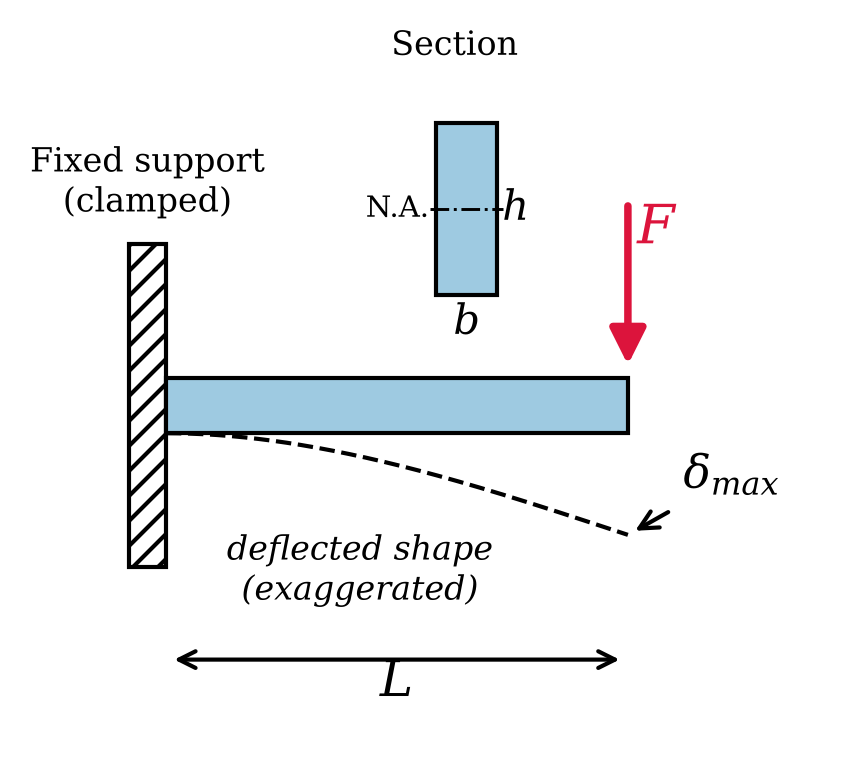
\includegraphics[width=0.62\textwidth]{06_beam_diagram.png}
\caption{Problem definition: prismatic cantilever of length $L$ and rectangular $b\times h$ section, clamped at $x=0$,
with a transverse point force $F$ at the free end. The maximum bending moment $M=FL$ acts at the support; the maximum
deflection occurs at the tip.}
\label{fig:beam}
\end{figure}

Euler--Bernoulli theory assumes that plane cross-sections remain plane and perpendicular to the deformed neutral axis,
so the axial strain varies linearly through the depth and shear deformation is neglected~\cite{gere2013}. The theory is
accurate for slender beams (span-to-depth ratio of roughly ten or more) under small deflections. The assumptions
adopted throughout are:
\begin{itemize}
\item linear-elastic, homogeneous, isotropic material (Hooke's law, $\sigma=E\varepsilon$);
\item small deflections and rotations (geometrically linear);
\item static load applied at the tip, no self-weight;
\item prismatic rectangular cross-section bending about its strong or weak axis as defined by $h$;
\item no stress concentrations, residual stresses, or support compliance;
\item failure is represented only by the onset of yield at the most stressed fibre.
\end{itemize}
The yield check compares the nominal elastic stress with the yield strength, the usual first design check for ductile
members under static load~\cite{budynas2015}. It does \emph{not} address fatigue, buckling (including lateral--torsional
buckling of tall narrow sections), fracture, plastic collapse or dynamic effects.

%==================================================================== MATH FORMULATION
\section{Mathematical formulation}
With $x$ measured from the fixed end, the bending moment and second moment of area are
\begin{equation}
M(x)=F\,(L-x),\qquad I=\frac{b h^{3}}{12}.
\end{equation}
The flexure formula gives the axial stress at height $y$ above the neutral axis,
\begin{equation}
\sigma_{xx}(x,y)=\frac{M(x)\,y}{I},
\end{equation}
which is largest at the support ($x=0$) on the outer fibres ($|y|=h/2$):
\begin{equation}
\boxed{\;\smax=\frac{F L\,(h/2)}{b h^{3}/12}=\frac{6FL}{bh^{2}}\;}
\label{eq:stress}
\end{equation}
Integrating $EI\,w''=M$ with $w(0)=w'(0)=0$ gives the elastic curve and tip deflection
\begin{equation}
w(x)=\frac{F x^{2}(3L-x)}{6EI},\qquad
\boxed{\;\dmax=w(L)=\frac{FL^{3}}{3EI}=\frac{4FL^{3}}{Ebh^{3}}\;}
\label{eq:defl}
\end{equation}
The maximum strain, factor of safety and yield label follow as
\begin{equation}
\varepsilon_{\max}=\frac{\smax}{E},\qquad \mathrm{FoS}=\frac{\sigma_y}{\smax},\qquad
y_{\mathrm{cls}}=\begin{cases}0 & \mathrm{FoS}\ge 1\ \text{(safe under the adopted criterion)}\\ 1 & \mathrm{FoS}<1\ \text{(yield criterion exceeded)}\end{cases}
\end{equation}

\paragraph{Power-law structure.} Equations~\eqref{eq:stress}--\eqref{eq:defl} are products of powers of the inputs.
Taking logarithms makes them exactly linear:
\begin{align}
\log\smax &= \log 6 + \log F + \log L - \log b - 2\log h,\\
\log\dmax &= \log 4 + \log F + 3\log L - \log E - \log b - 3\log h.
\end{align}
This fact drives two design decisions: models are trained on $\log_{10}$ targets, and a linear least-squares fit in log
space is included as a physics-informed reference model. The exponents also give exact \emph{elasticities}
$\partial\ln y/\partial\ln x_i$ against which learned sensitivities are tested (Section~\ref{sec:sens}).

\begin{figure}[H]\centering
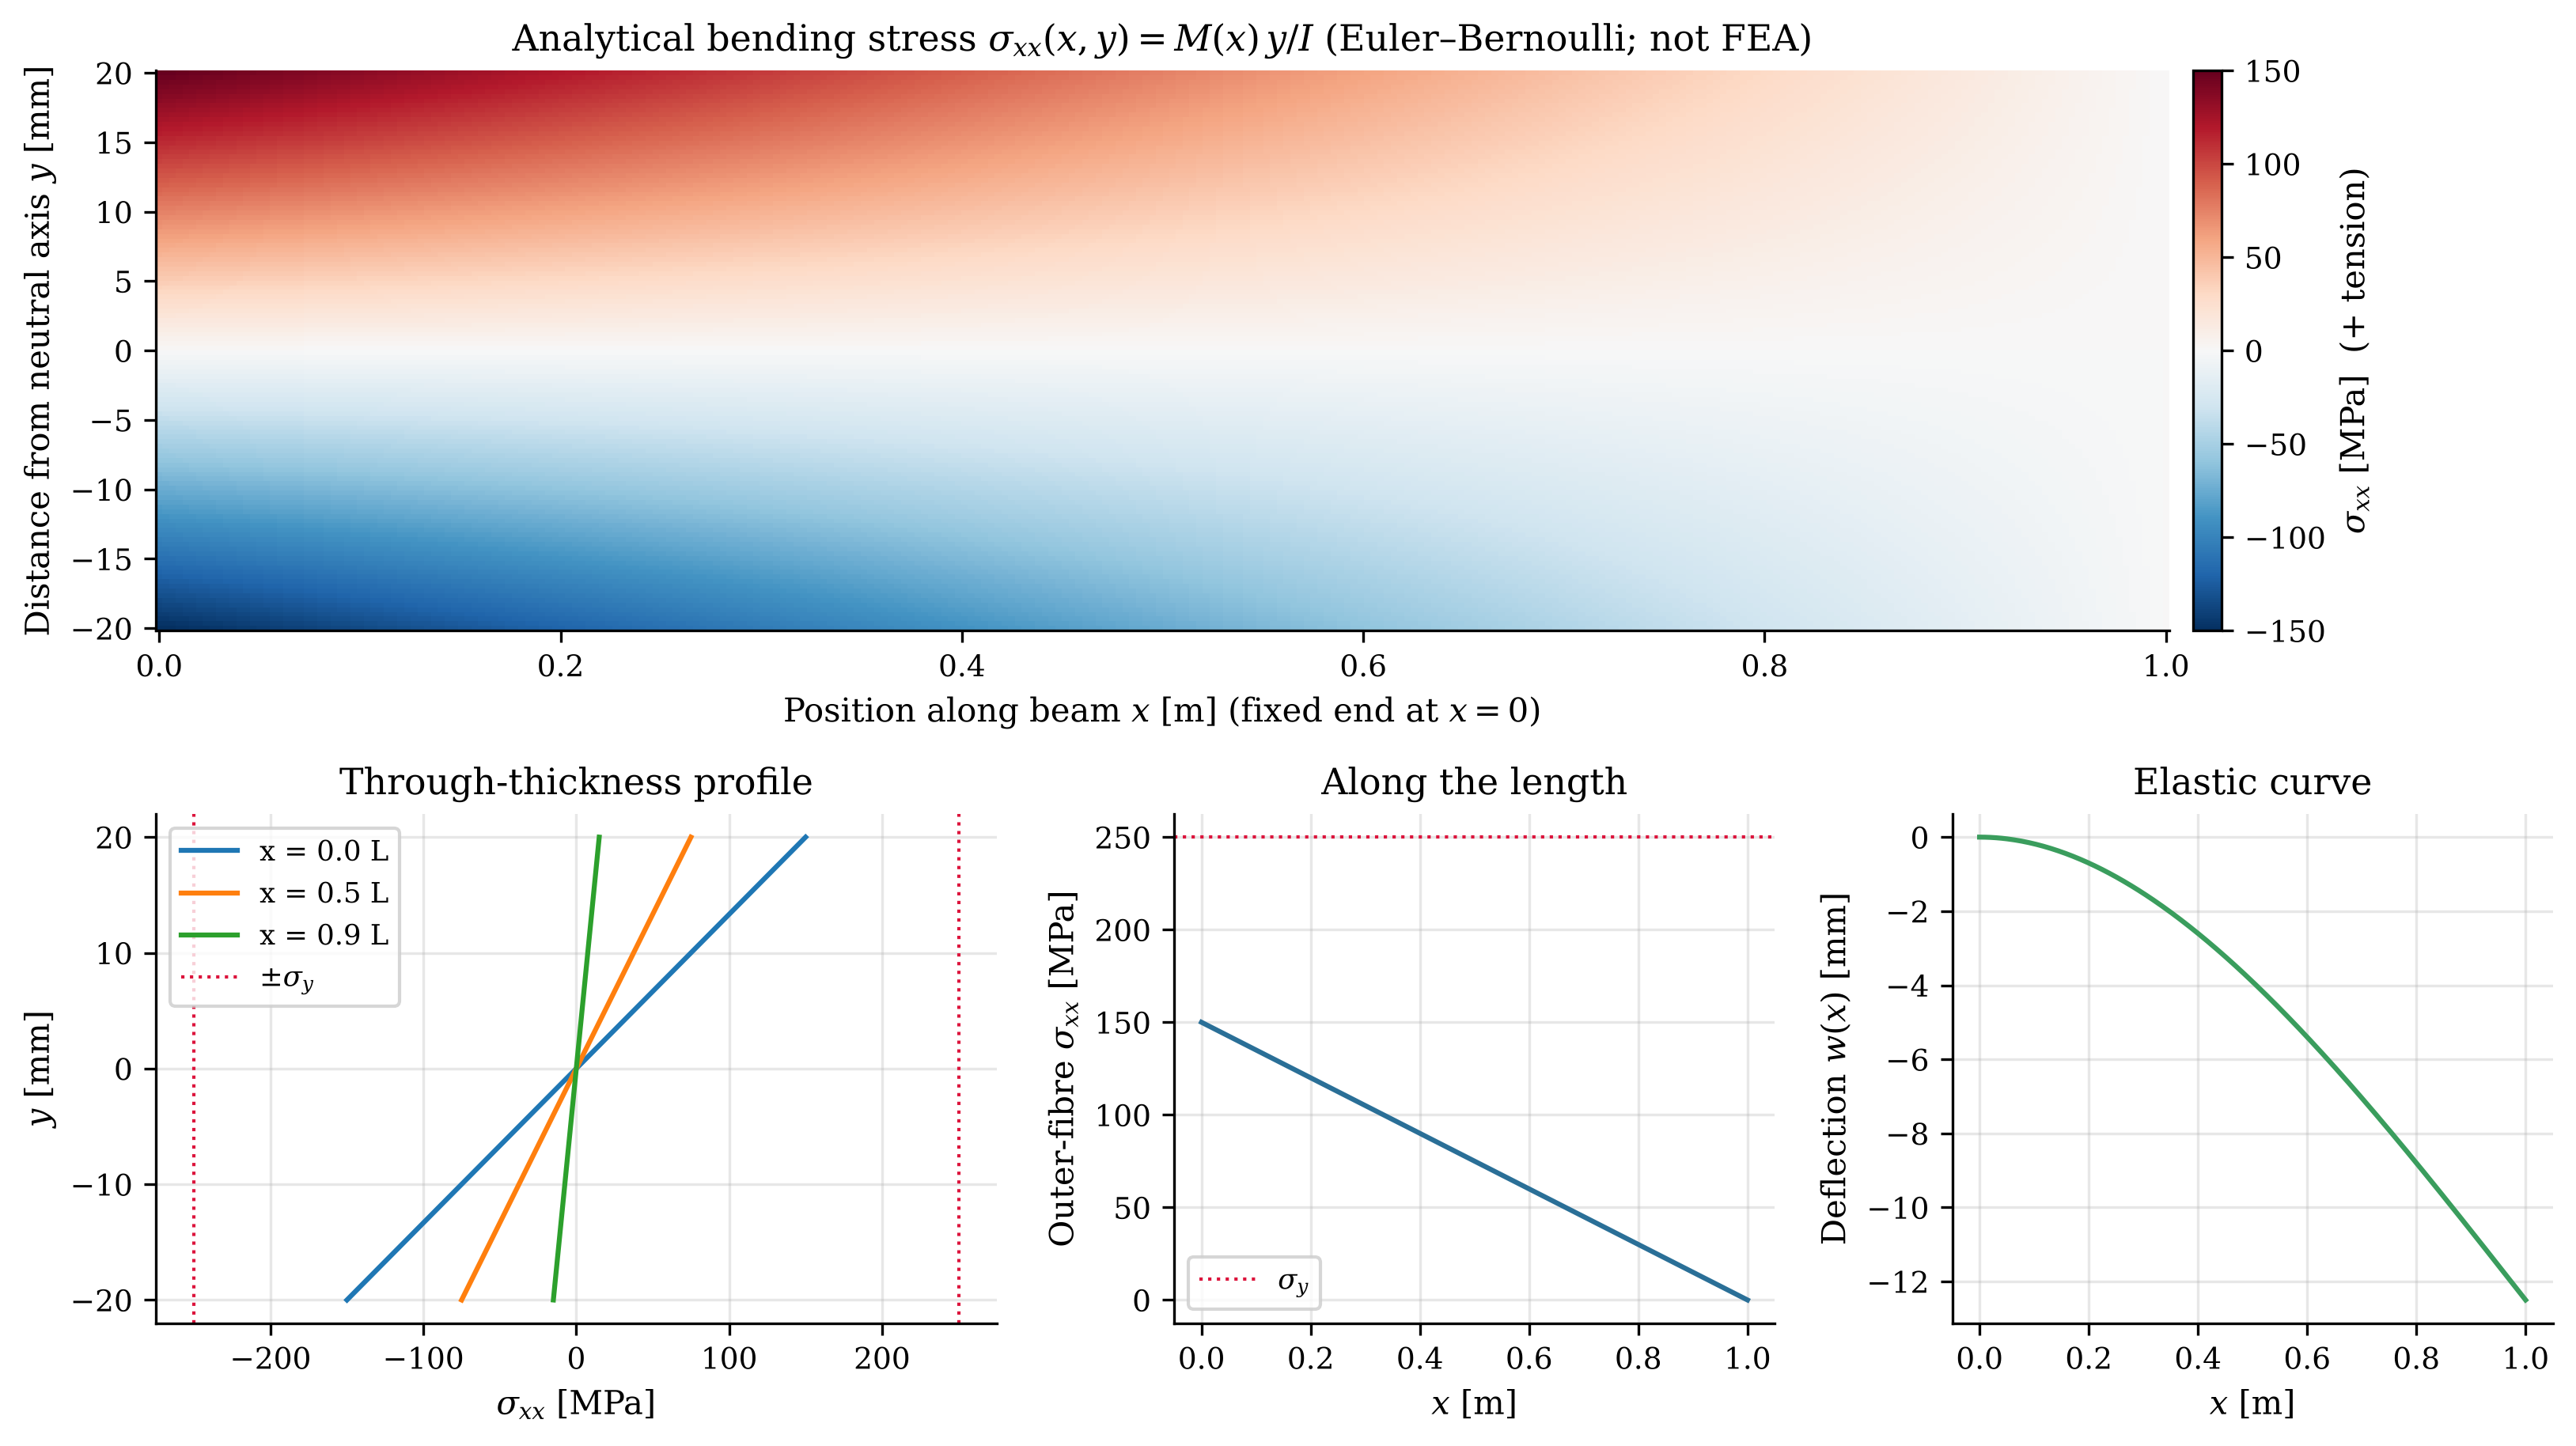
\includegraphics[width=\textwidth]{07_bending_stress_field.png}
\caption{Analytical fields for the baseline beam ($L=1$\,m, $b=50$\,mm, $h=40$\,mm, $F=2$\,kN, $E=200$\,GPa,
$\sigma_y=250$\,MPa): bending stress over the beam (top), through-thickness profiles, outer-fibre stress along the
span, and the elastic curve. Peak stress is <<BASE_S>>\,MPa (FoS $=$ <<BASE_FOS>>) and tip deflection
<<BASE_D>>\,mm. These are closed-form beam-theory fields, \textbf{not} finite-element results; local effects near the
clamp are not represented.}
\label{fig:field}
\end{figure}

%==================================================================== DATASET
\section{Dataset generation}
\subsection{Sampling and physical-validity constraints}
The six inputs were sampled independently from uniform distributions (Table~\ref{tab:ranges}) using NumPy's
\texttt{default\_rng} with seed 42~\cite{harris2020}. Each candidate was evaluated with the analytical solver and kept
only if it satisfied three validity constraints:
\begin{enumerate}
\item $L/h\ge 10$: slender beam, consistent with neglecting shear deformation;
\item $\dmax/L\le 0.05$: small-deflection assumption;
\item $\smax/\sigma_y\le 3$: the nominal elastic stress is retained only as a screening quantity near the yield
boundary---beams loaded far into the plastic range, where an elastic stress has no physical meaning, are excluded.
\end{enumerate}
Of <<NDRAWN>> candidates, <<NACC>> (<<ACC_RATE>>\,\%) passed; the first <<N>> form the dataset. Automatic checks confirm
that there are no missing or non-finite values, all rows satisfy the constraints, all targets reproduce the solver to a
relative tolerance of $10^{-12}$, and there are no duplicate inputs.

\begin{table}[H]\centering\small
\caption{Input parameters, sampling ranges and resulting dataset statistics.}
\label{tab:ranges}
\begin{tabular}{llcccc}
\toprule
Parameter & Symbol & Unit & Sampling range & Mean & Median\\
\midrule
<<TABLE_INPUTS>>
\bottomrule
\end{tabular}
\end{table}

\subsection{Exploratory data analysis}
The rejection step makes the input distributions non-uniform (Figure~\ref{fig:dist}): long beams, thin beams, large forces
and low moduli are under-represented, because these combinations most often violate the deflection or stress limits.
It also introduces weak correlations between nominally independent inputs (e.g.\ Pearson $r(h,F)=<<R_HF>>$,
$r(L,F)=<<R_LF>>$; Figure~\ref{fig:corr}). <<YIELD_PCT>>\,\% of beams exceed the yield criterion, giving a moderately
imbalanced classification problem. Responses span two to three orders of magnitude (Figure~\ref{fig:targets}).
IQR-rule ``outliers'' in the log-transformed targets (<<IQR_S>> for stress, <<IQR_D>> for deflection) are genuine extreme
configurations rather than errors and were retained.

\begin{figure}[H]\centering
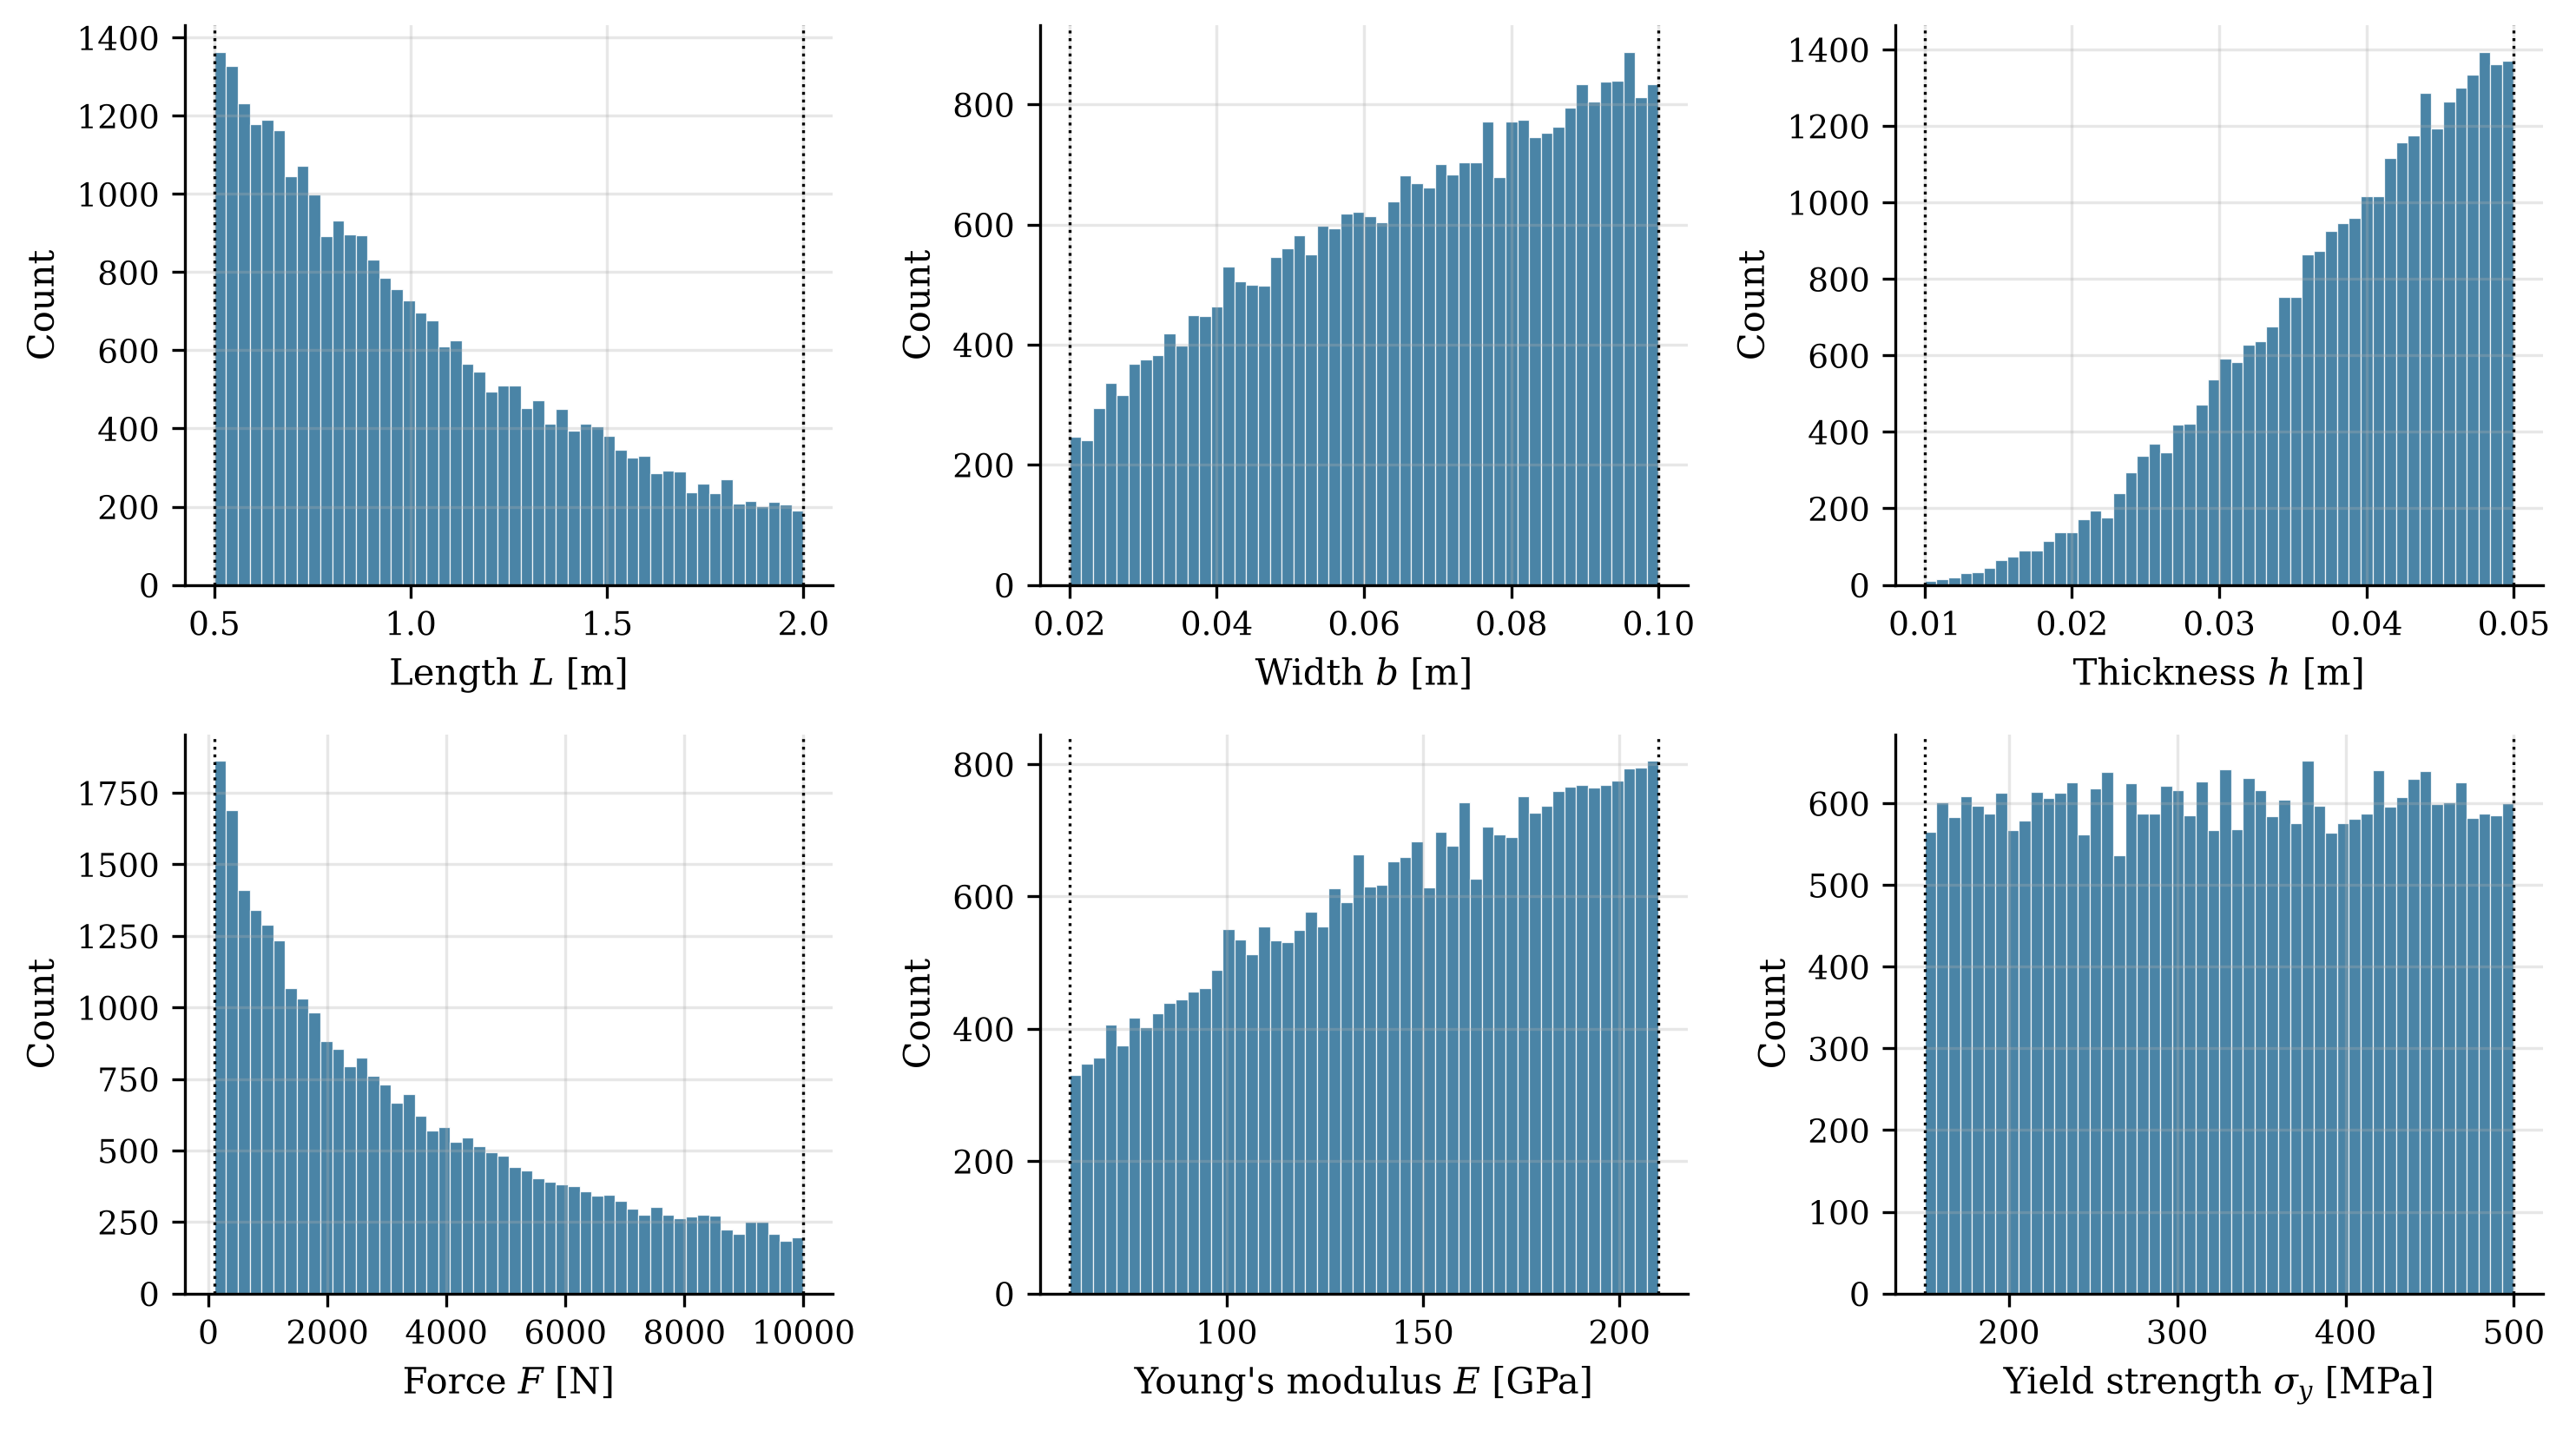
\includegraphics[width=0.92\textwidth]{01_feature_distributions.png}
\caption{Input distributions after rejection sampling; dotted lines are the sampling bounds.}
\label{fig:dist}
\end{figure}
\begin{figure}[H]\centering
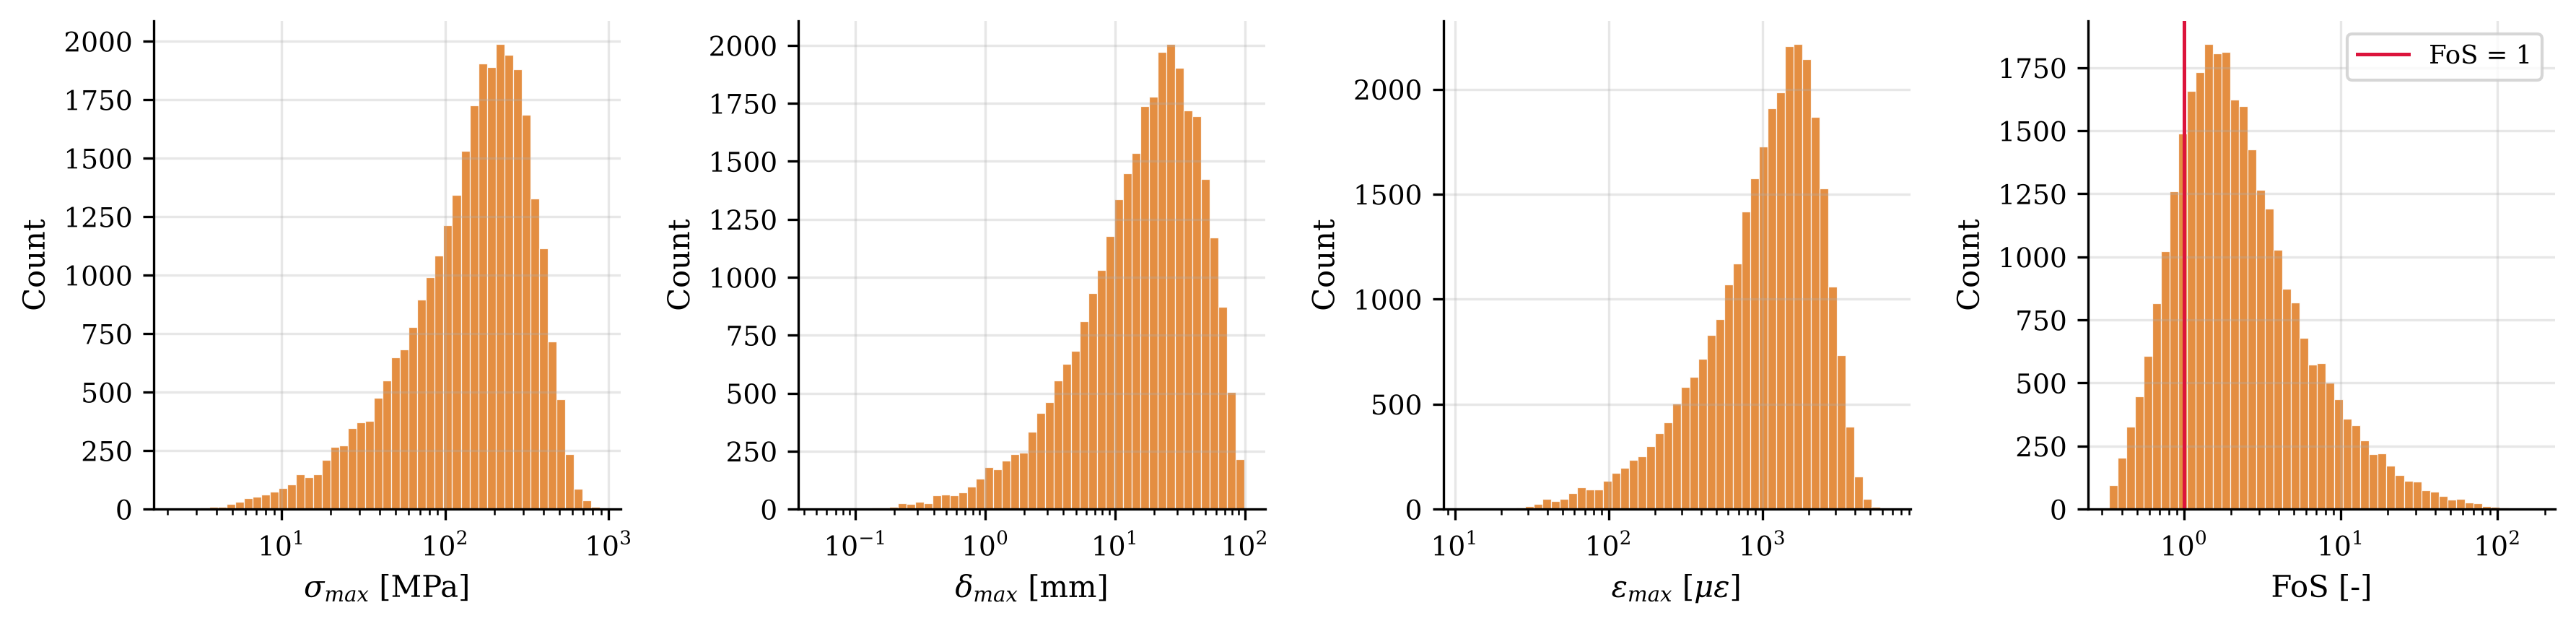
\includegraphics[width=\textwidth]{02_target_distributions.png}
\caption{Distributions of the analytical responses (log axes). The red line marks FoS $=1$.}
\label{fig:targets}
\end{figure}
\begin{figure}[H]\centering
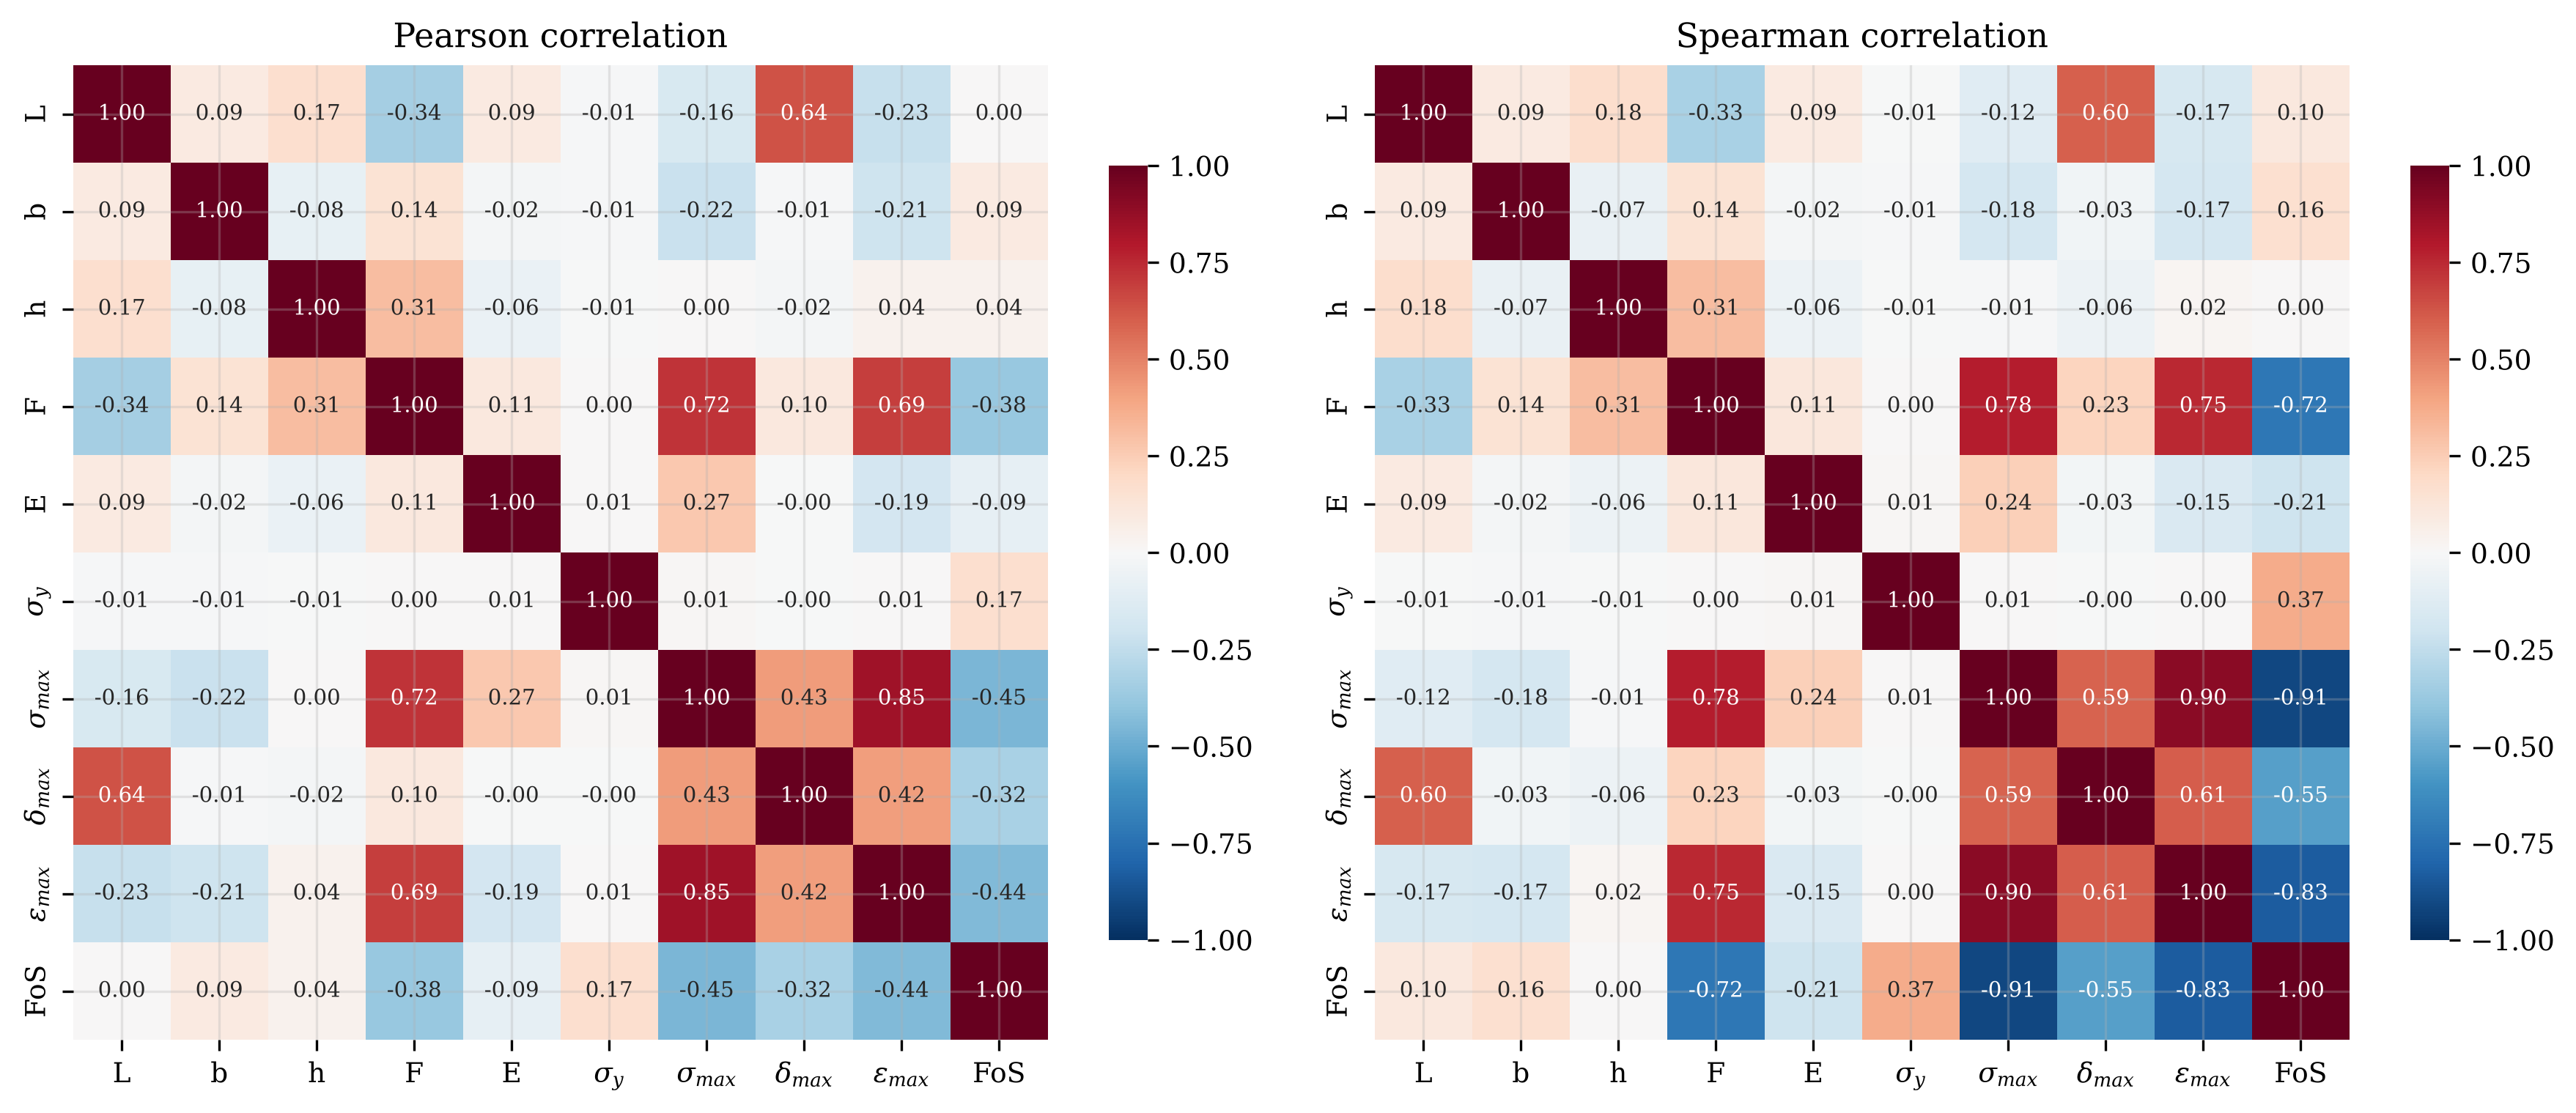
\includegraphics[width=\textwidth]{03_correlation_heatmap.png}
\caption{Pearson and Spearman correlation matrices of inputs and responses. Force is the input most strongly correlated
with stress; length with deflection.}
\label{fig:corr}
\end{figure}
\begin{figure}[H]\centering
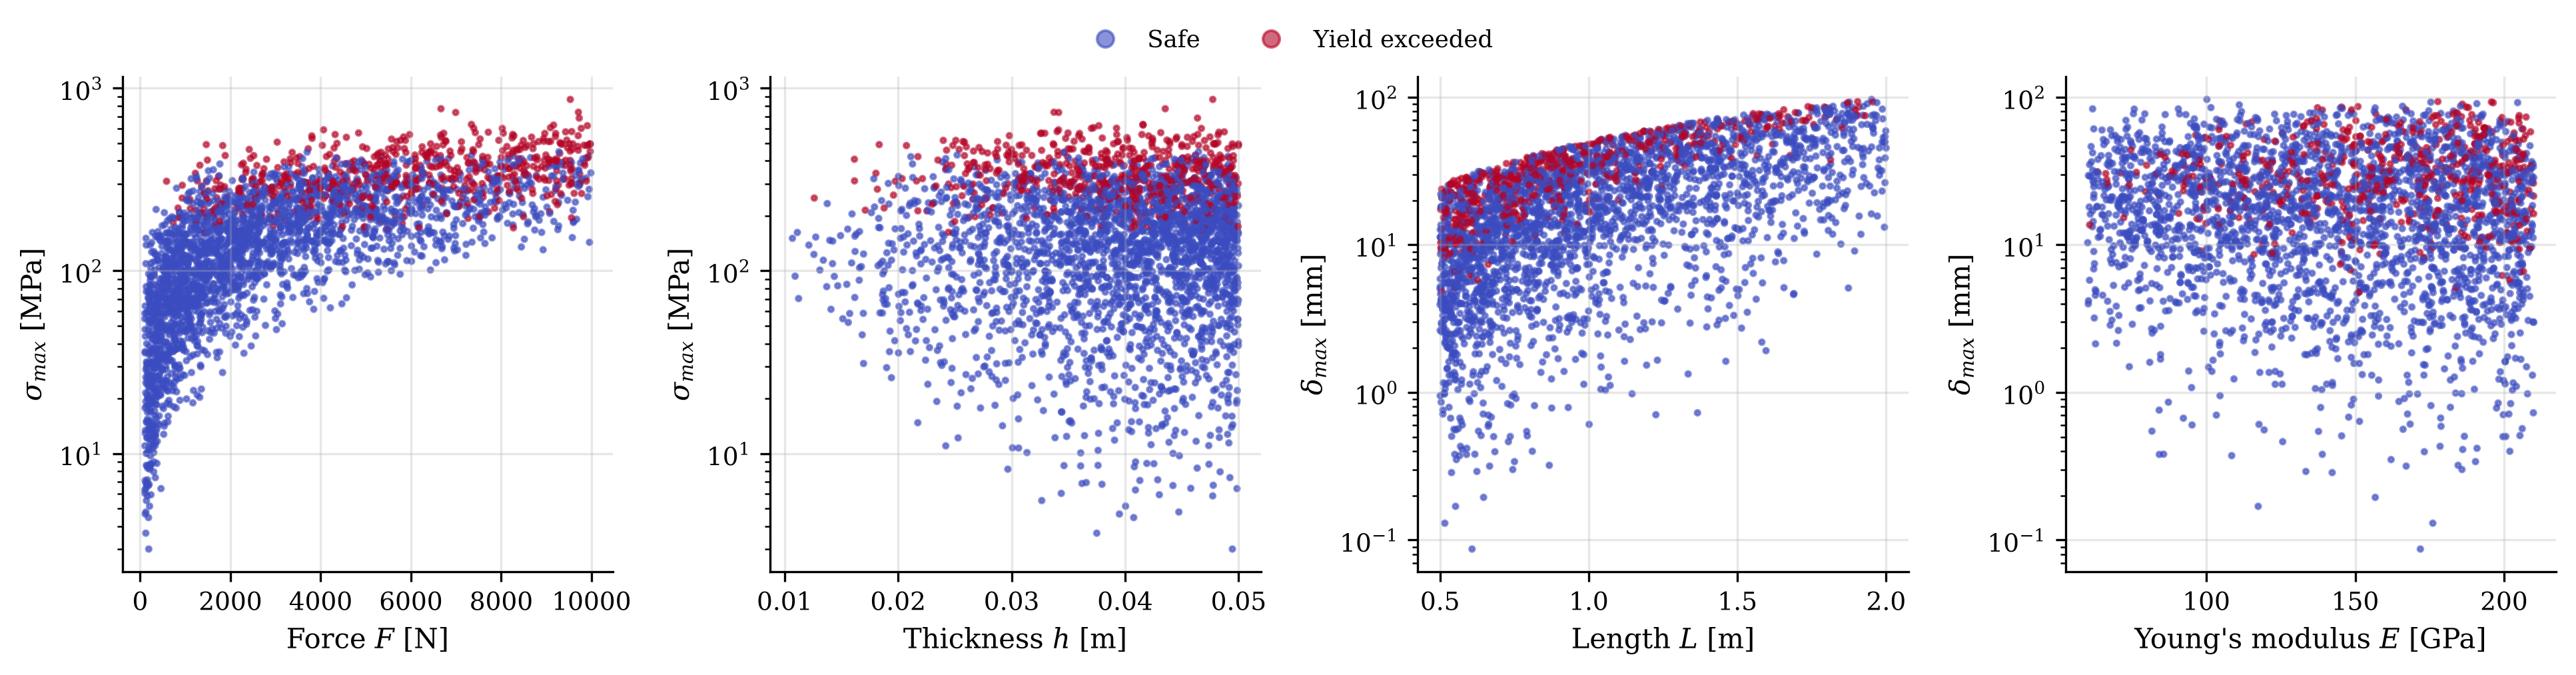
\includegraphics[width=\textwidth]{04_feature_relationships.png}
\caption{Marginal input--response relationships for 3\,000 random samples (colour: yield class). The wide scatter at
fixed input shows that each response depends jointly on several parameters.}
\end{figure}

%==================================================================== ML METHODOLOGY
\section{Machine learning methodology}
\subsection{Data representation}
Stress and deflection are strictly positive and span several decades, so all regressors learn
$\log_{10}\smax$ and $\log_{10}\dmax$; predictions are transformed back to SI units before any metric is computed.
Strain and FoS are \emph{derived} from the predicted stress and the known inputs ($\varepsilon=\hat\sigma/E$,
$\widehat{\mathrm{FoS}}=\sigma_y/\hat\sigma$) rather than learned separately, which keeps the four outputs mutually
consistent.

\subsection{Models}
\begin{description}
\item[Random forest~\cite{breiman2001}.] Bagged ensemble of deep regression trees with a two-output target. Tree
ensembles are invariant to monotone transformations of inputs, so raw SI features are used.
\item[Gradient-boosted trees~\cite{friedman2001}.] <<GB_DESC>>
\item[Multi-layer perceptron~\cite{hornik1989}.] <<MLP_DESC>> Inputs are $\log_{10}$-transformed and standardised
with statistics from the training split only; targets are standardised log values.
\item[Power-law reference.] Ordinary least squares on $\log_{10}$ inputs. Because the true model is exactly linear in
this space, this reference is expected to be exact; it is reported to make that explicit, not as a competing ``ML'' method.
\item[MLP ablation (raw inputs).] Identical MLP trained on linearly standardised (not log-transformed) inputs, to
measure the value of the log representation.
\end{description}
For classification of the yield criterion, a random-forest classifier, a gradient-boosted classifier and an MLP
classifier were trained directly on the six inputs. In addition, a \emph{derived} classifier thresholds the FoS implied by
each stress regressor.

\subsection{Hyper-parameter selection}
A small grid was searched for each model family, selecting on the validation-set RMSE of the $\log_{10}$ targets
(Table~\ref{tab:hp}). The test split was not used for any choice.
\begin{table}[H]\centering\footnotesize
\caption{Hyper-parameter grids and selected values (validation RMSE in $\log_{10}$ units, averaged over both targets).}
\label{tab:hp}
\begin{tabular}{p{2.6cm}p{6.6cm}p{5.4cm}}
\toprule
Model & Grid searched & Selected (validation RMSE)\\
\midrule
<<TABLE_HP>>
\bottomrule
\end{tabular}
\end{table}

%==================================================================== EXPERIMENTAL SETUP
\section{Experimental setup}
\begin{itemize}
\item \textbf{Split:} 70/15/15\,\% train/validation/test (<<NTRAIN>>/<<NVAL>>/<<NTEST>> beams), stratified on the yield
label, seed 42. Feature scaling and target scaling are fitted on the training split only.
\item \textbf{Regression metrics:} MAE, RMSE and $R^2$ in SI units, plus absolute percentage error (APE) statistics
(mean, median, 95th percentile, maximum), which are more informative for targets spanning several decades.
\item \textbf{Classification metrics:} accuracy, precision, recall, $F_1$ (positive class $=$ yield exceeded), ROC-AUC
and confusion matrices.
\item \textbf{Extrapolation test:} models retrained on beams with $F\le$ <<OOD_THR>>\,N (85th percentile of $F$;
<<OOD_NTR>> beams) and evaluated on the <<OOD_NTE>> beams with larger force.
\item \textbf{Sensitivity analysis:} one-at-a-time sweeps around the baseline beam and global variance shares (Section~\ref{sec:sens}).
\item \textbf{Reproducibility:} every stage is scripted (scikit-learn~\cite{pedregosa2011}, Matplotlib~\cite{hunter2007}); \texttt{python run\_pipeline.py} regenerates the dataset,
models, metrics and figures, then runs 11 automated tests including hand-calculated solver checks and a test that
re-scores reloaded models and compares the result with the saved metrics. Two full runs from an empty directory
produced the same dataset and models; with single-threaded forest inference, repeated evaluations give bit-identical metrics. Compute: 2 CPU cores, no GPU; the timed regression-training stages took <<TRAIN_TIME>>\,s in total.
\end{itemize}

%==================================================================== RESULTS
\section{Model evaluation}
\subsection{Regression}
\begin{table}[H]\centering\footnotesize\setlength{\tabcolsep}{4pt}
\caption{Test-set regression metrics ($N=$ <<NTEST>>). MAE and RMSE are in MPa for stress and mm for deflection.
APE: absolute percentage error. Best ML model per column in bold.}
\label{tab:reg}
\begin{tabular}{llrrrrrr}
\toprule
Target & Model & MAE & RMSE & $R^2$ & Median APE\,\% & P95 APE\,\% & Max APE\,\%\\
\midrule
<<TABLE_REG>>
\bottomrule
\end{tabular}
\end{table}

\begin{figure}[H]\centering
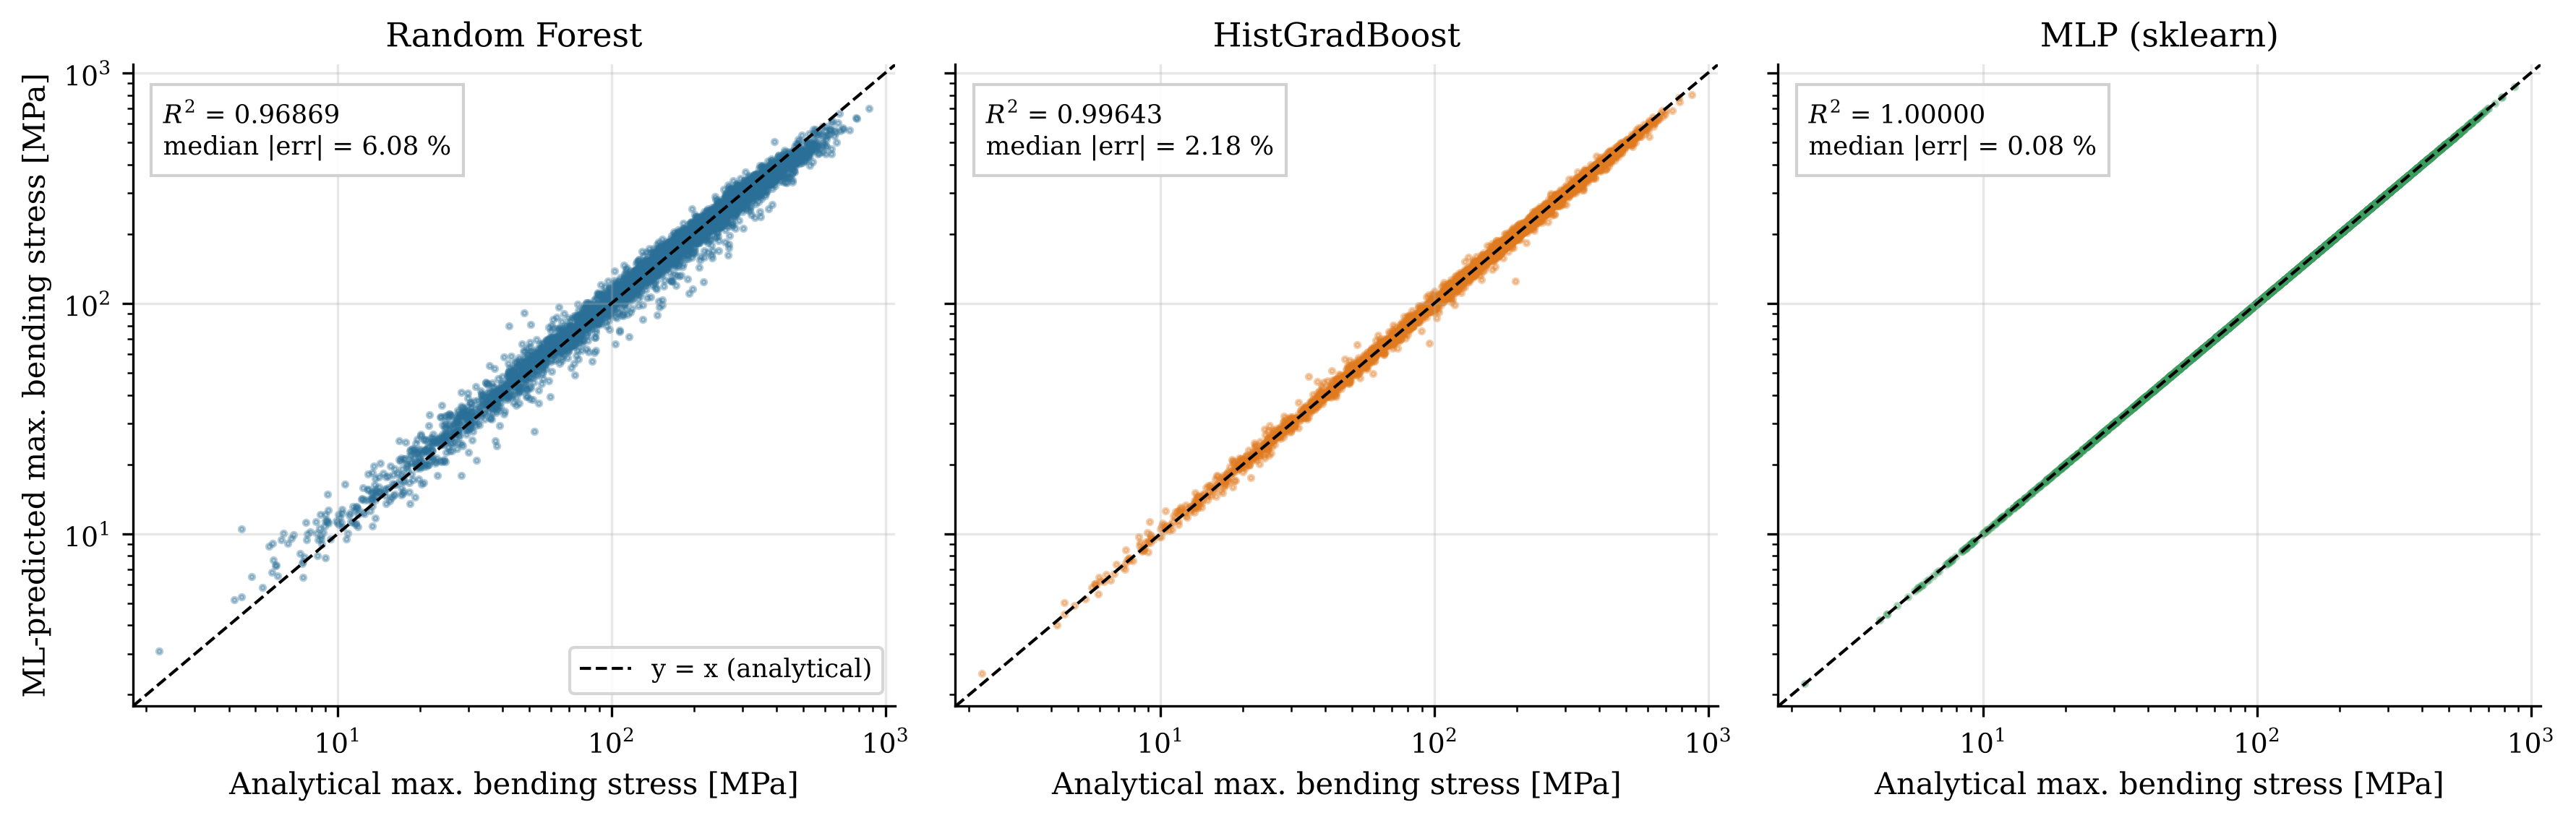
\includegraphics[width=\textwidth]{09_pred_vs_actual_stress.png}
\caption{Predicted versus analytical maximum bending stress on the test set (log--log axes).}
\label{fig:pva_s}
\end{figure}
\begin{figure}[H]\centering
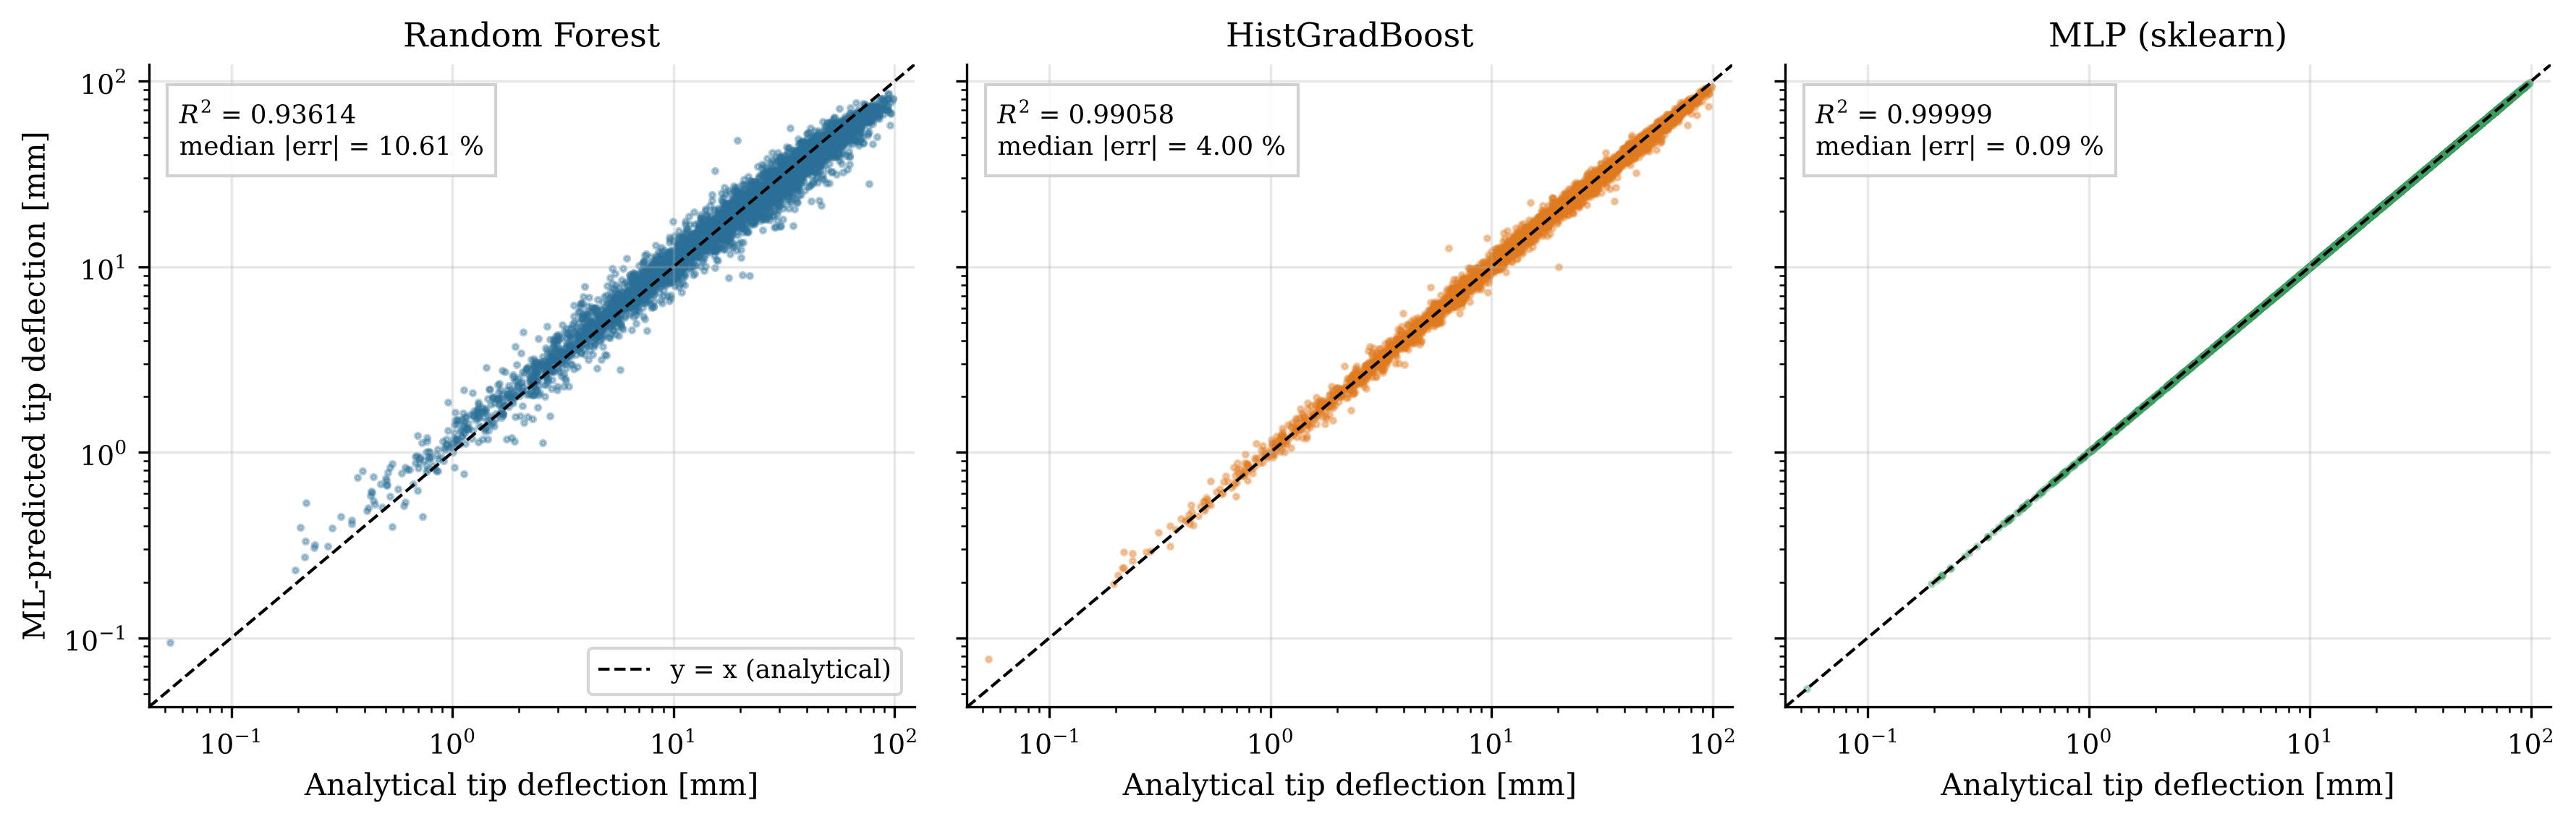
\includegraphics[width=\textwidth]{10_pred_vs_actual_deflection.png}
\caption{Predicted versus analytical tip deflection on the test set (log--log axes).}
\end{figure}
\begin{figure}[H]\centering
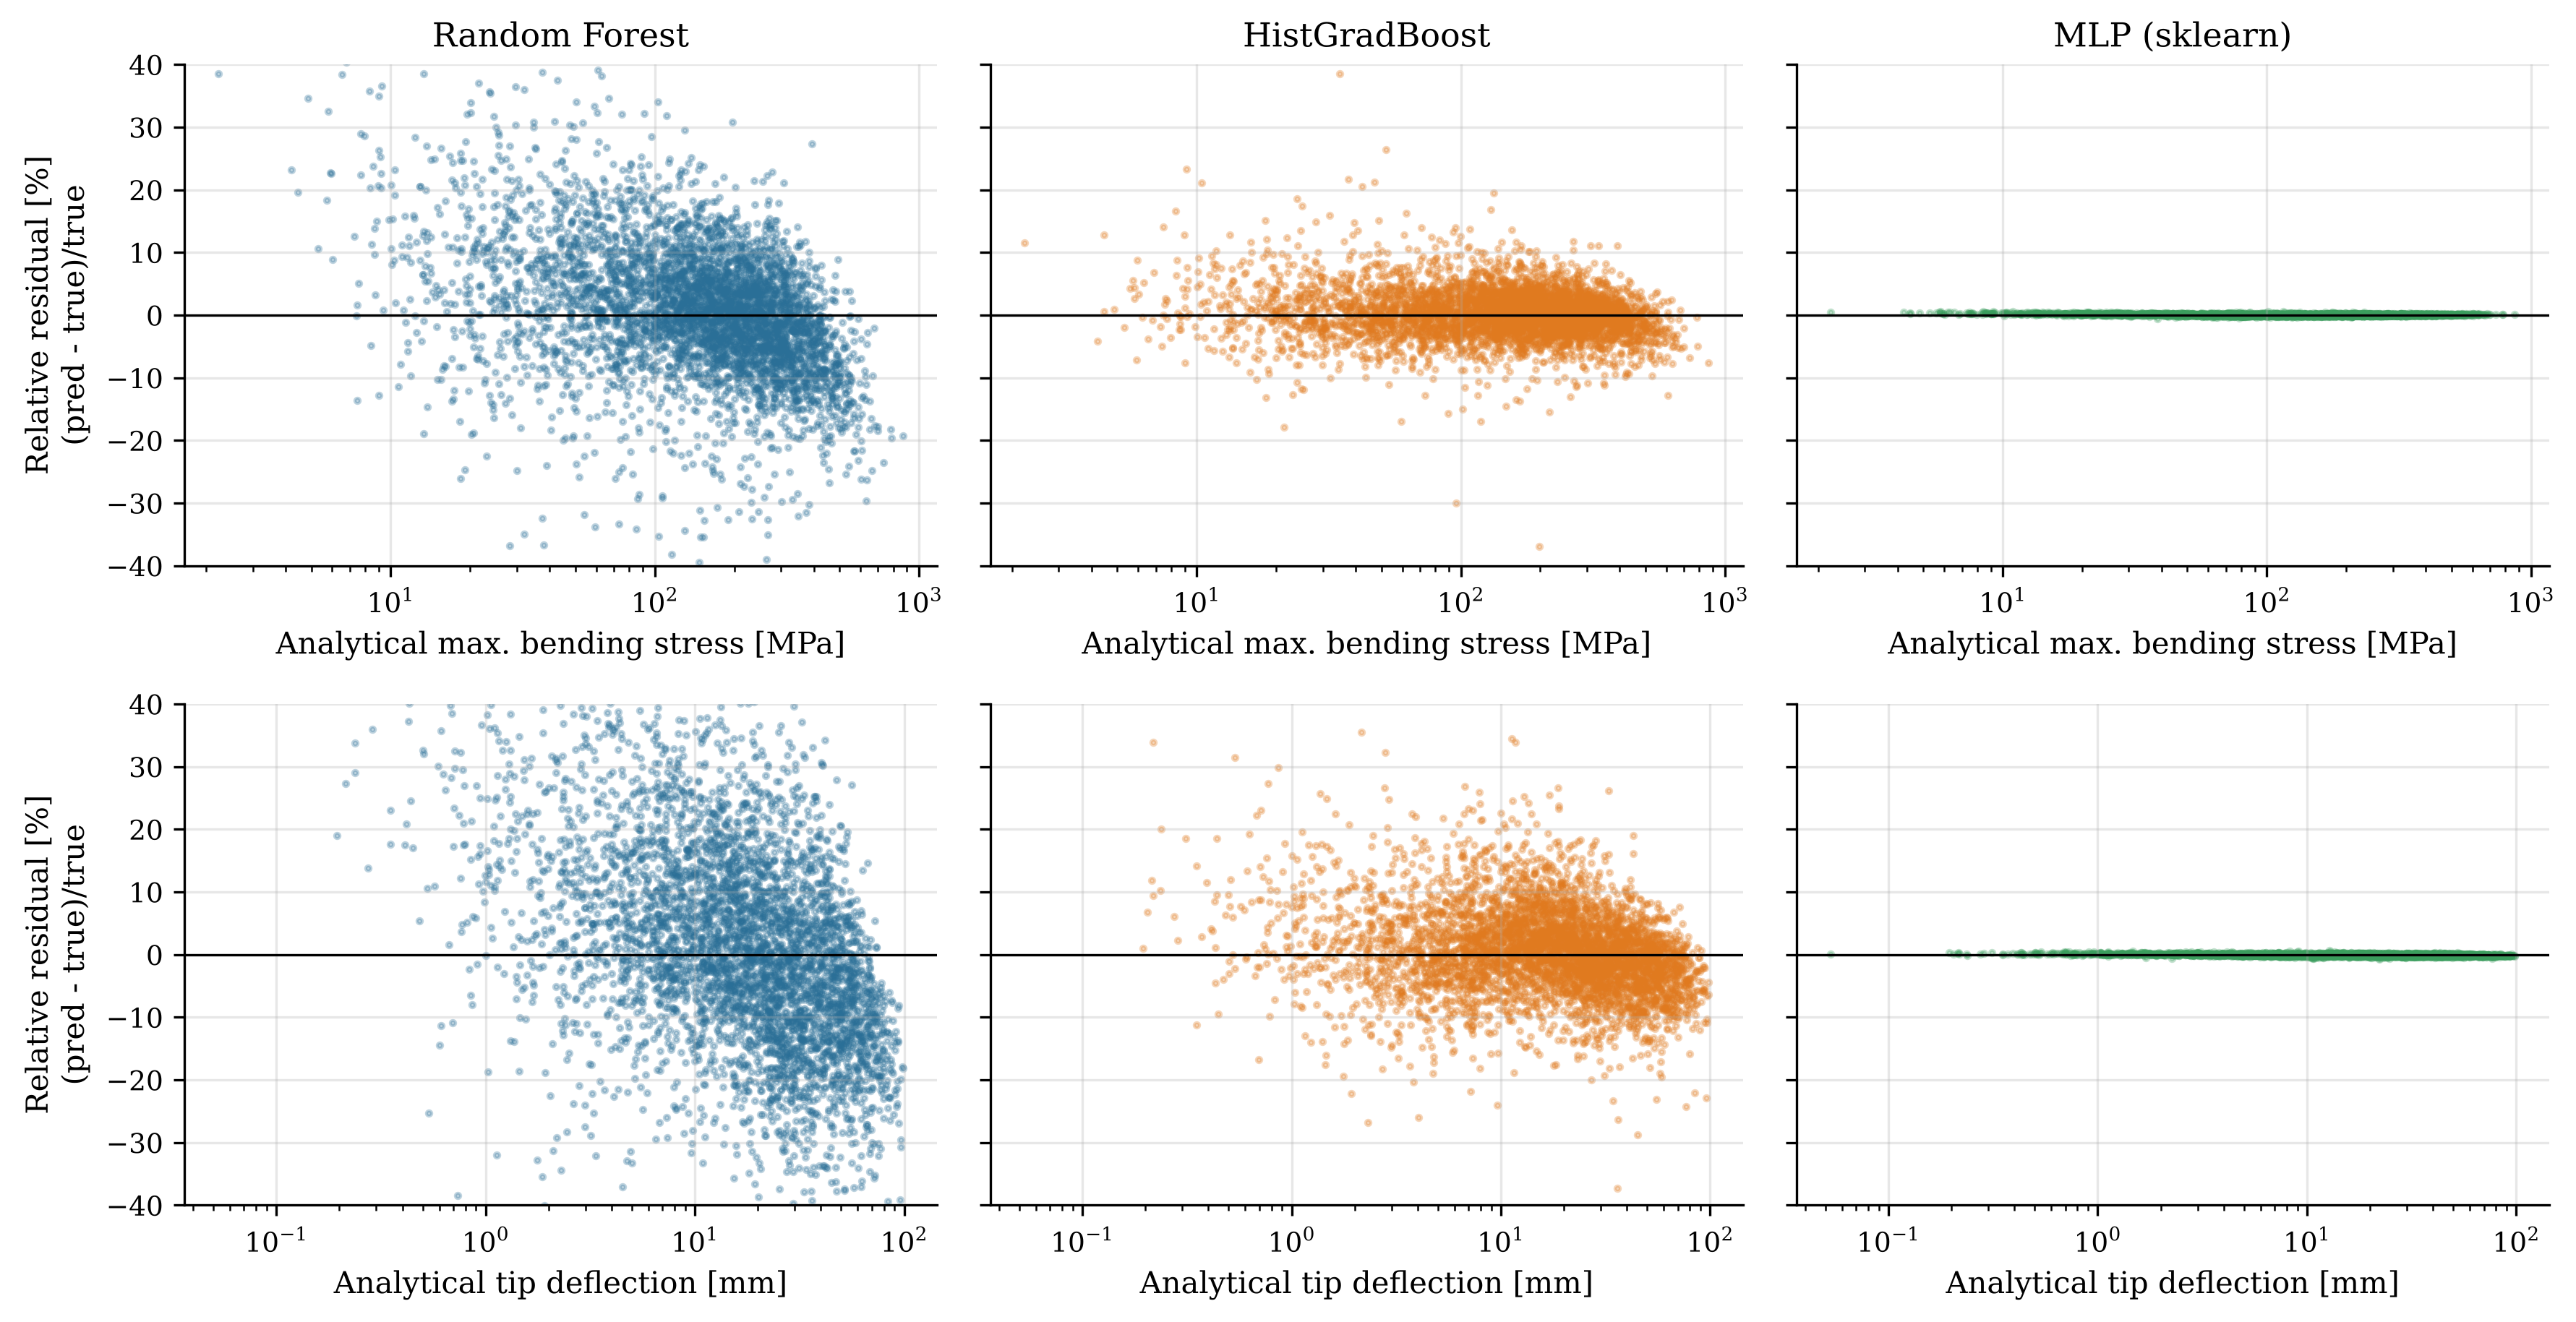
\includegraphics[width=\textwidth]{11_residuals.png}
\caption{Relative residuals versus analytical value (axes clipped at $\pm40$\,\%). Tree-ensemble errors are
largest at the extremes of the target range, where training data are sparse.}
\label{fig:resid}
\end{figure}
\begin{figure}[H]\centering
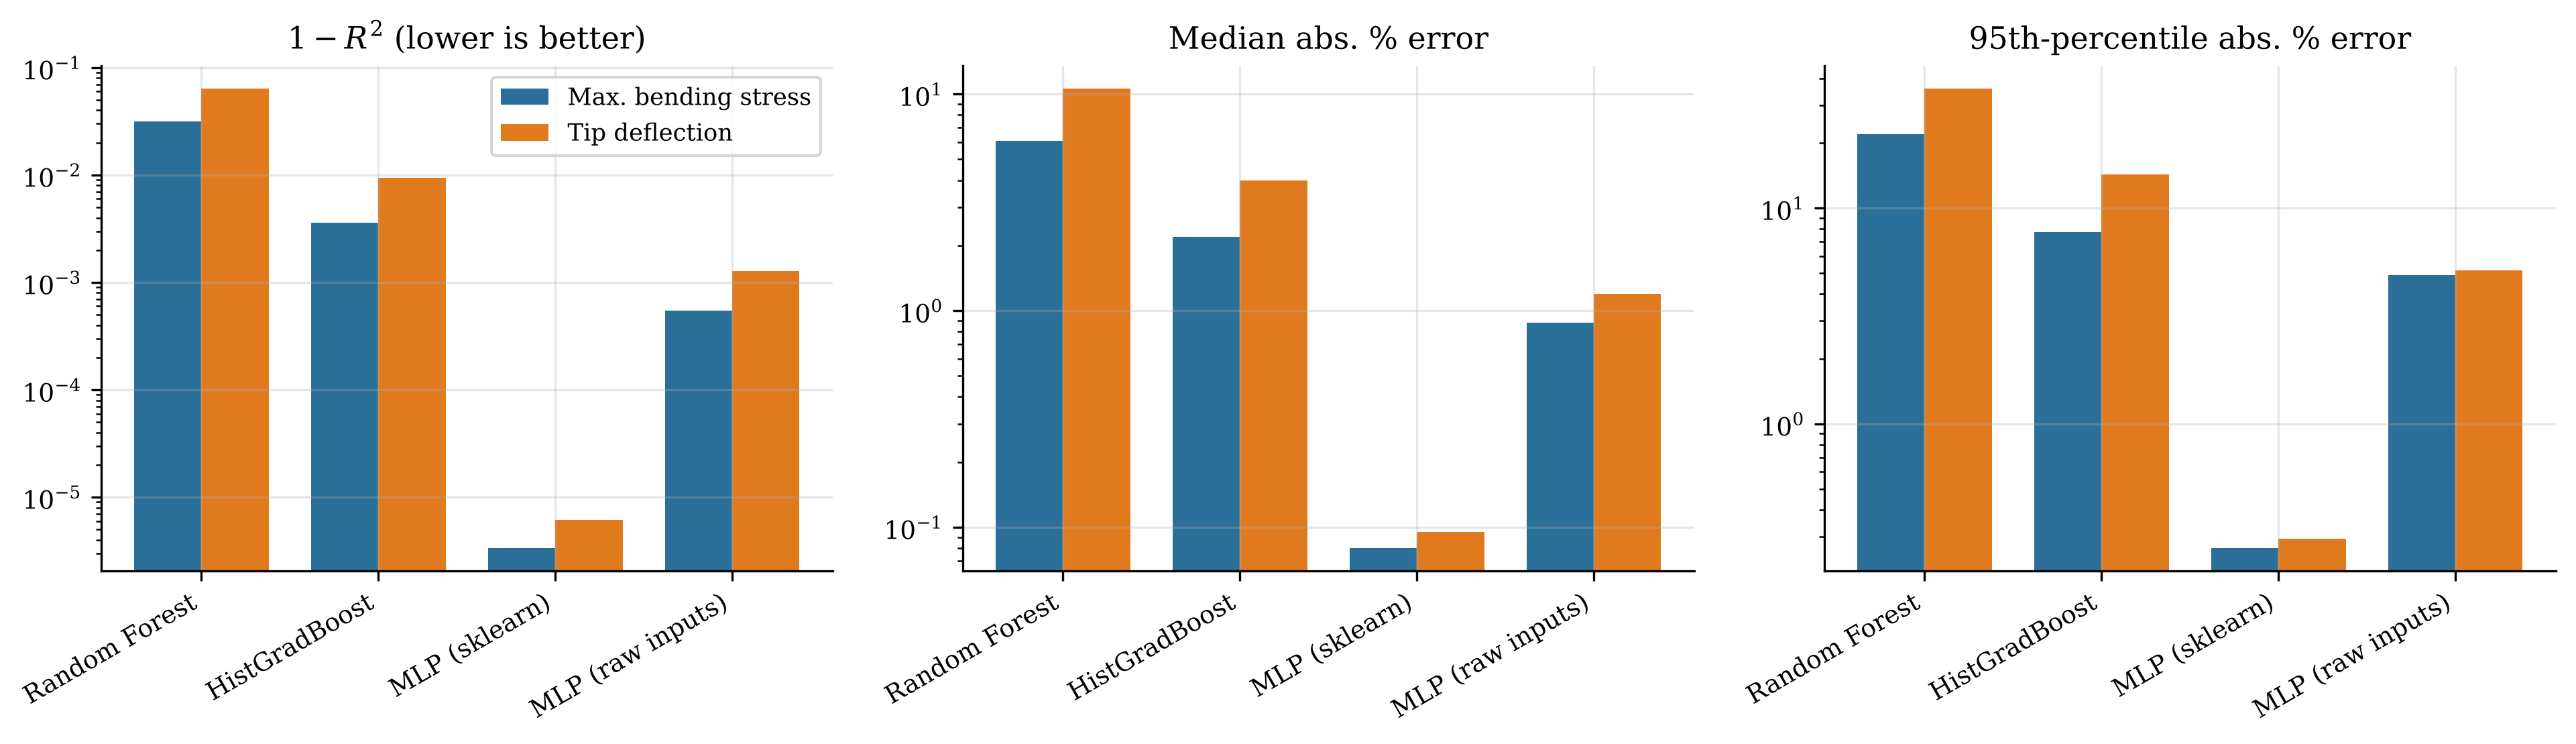
\includegraphics[width=\textwidth]{12_model_comparison.png}
\caption{Test-set comparison of regressors (log scale). The power-law reference is omitted because its errors are at
machine precision (median APE $\sim10^{-12}$\,\%).}
\label{fig:compare}
\end{figure}

\subsection{Yield classification}
\begin{table}[H]\centering\small
\caption{Test-set yield-classification metrics (positive class: FoS $<1$; <<NPOS>> positives of <<NTEST>>).}
\label{tab:cls}
\begin{tabular}{lrrrrr}
\toprule
Classifier & Accuracy & Precision & Recall & $F_1$ & ROC-AUC\\
\midrule
<<TABLE_CLS>>
\bottomrule
\end{tabular}
\end{table}
\begin{figure}[H]\centering
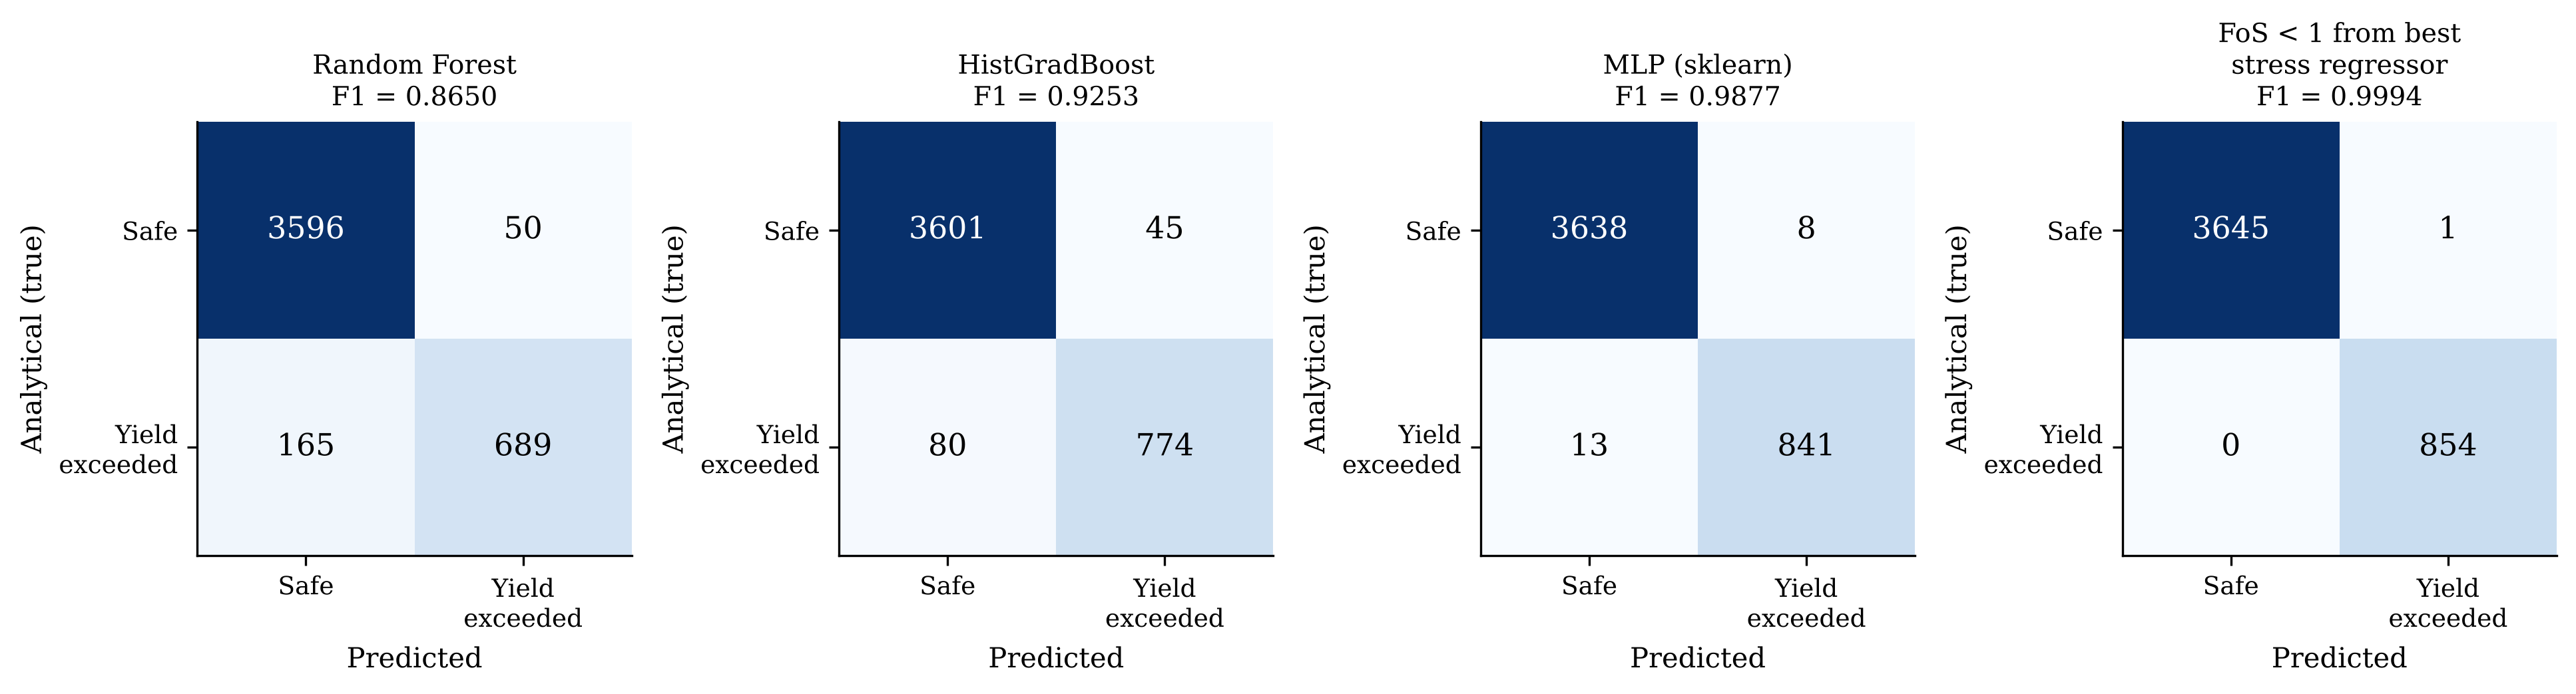
\includegraphics[width=\textwidth]{13_confusion_matrices.png}
\caption{Confusion matrices: three direct classifiers and the classifier derived from the best stress regressor.}
\end{figure}
\begin{figure}[H]\centering
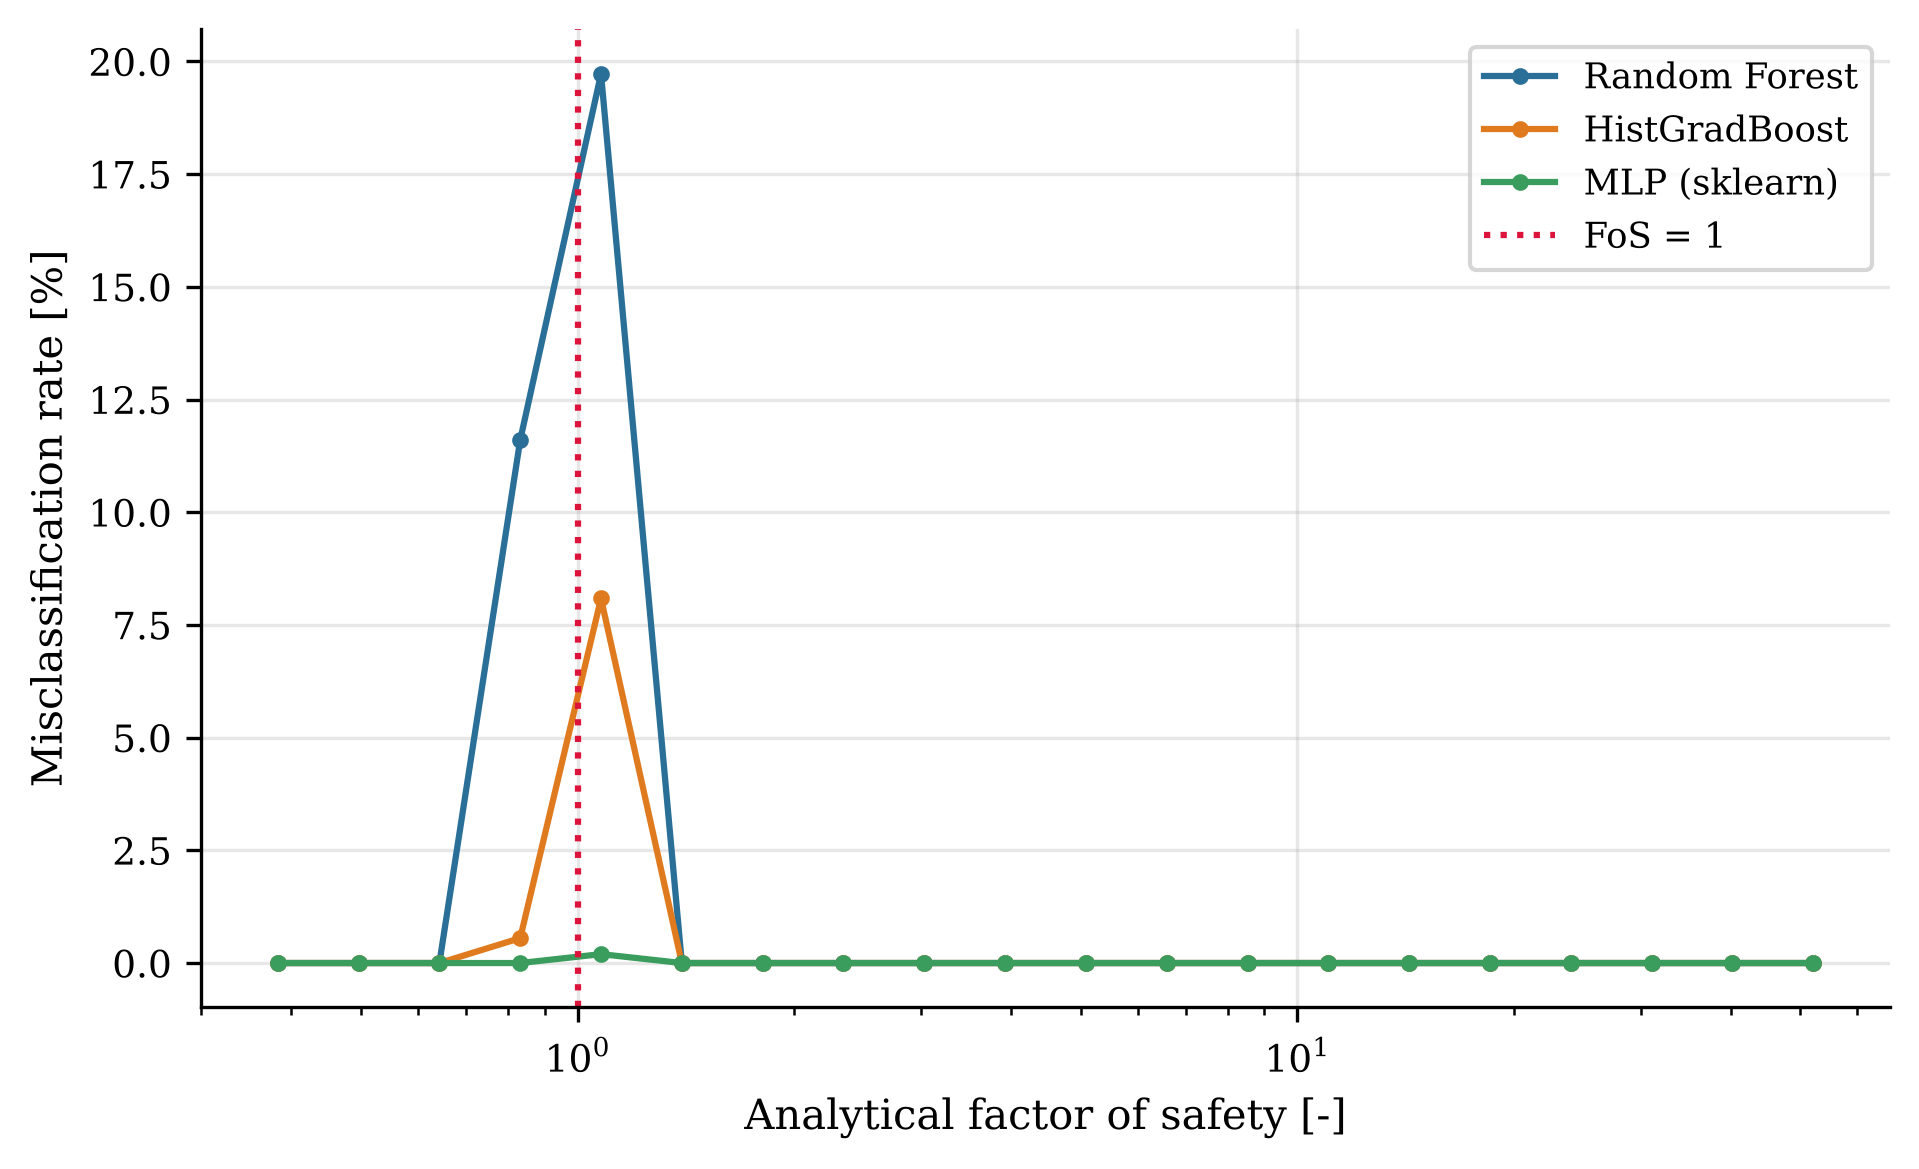
\includegraphics[width=0.62\textwidth]{14_fos_misclassification.png}
\caption{Misclassification rate of the regression-derived yield label, binned by true FoS.}
\label{fig:fosmis}
\end{figure}

\subsection{Extrapolation beyond the training range}
\begin{table}[H]\centering\small
\caption{Extrapolation test: trained on $F\le$ <<OOD_THR>>\,N, tested on larger forces (<<OOD_NTE>> beams).}
\label{tab:ood}
\begin{tabular}{lrrrr}
\toprule
& \multicolumn{2}{c}{Stress} & \multicolumn{2}{c}{Deflection}\\
Model & $R^2$ & Median APE\,\% & $R^2$ & Median APE\,\%\\
\midrule
<<TABLE_OOD>>
\bottomrule
\end{tabular}
\end{table}
\begin{figure}[H]\centering
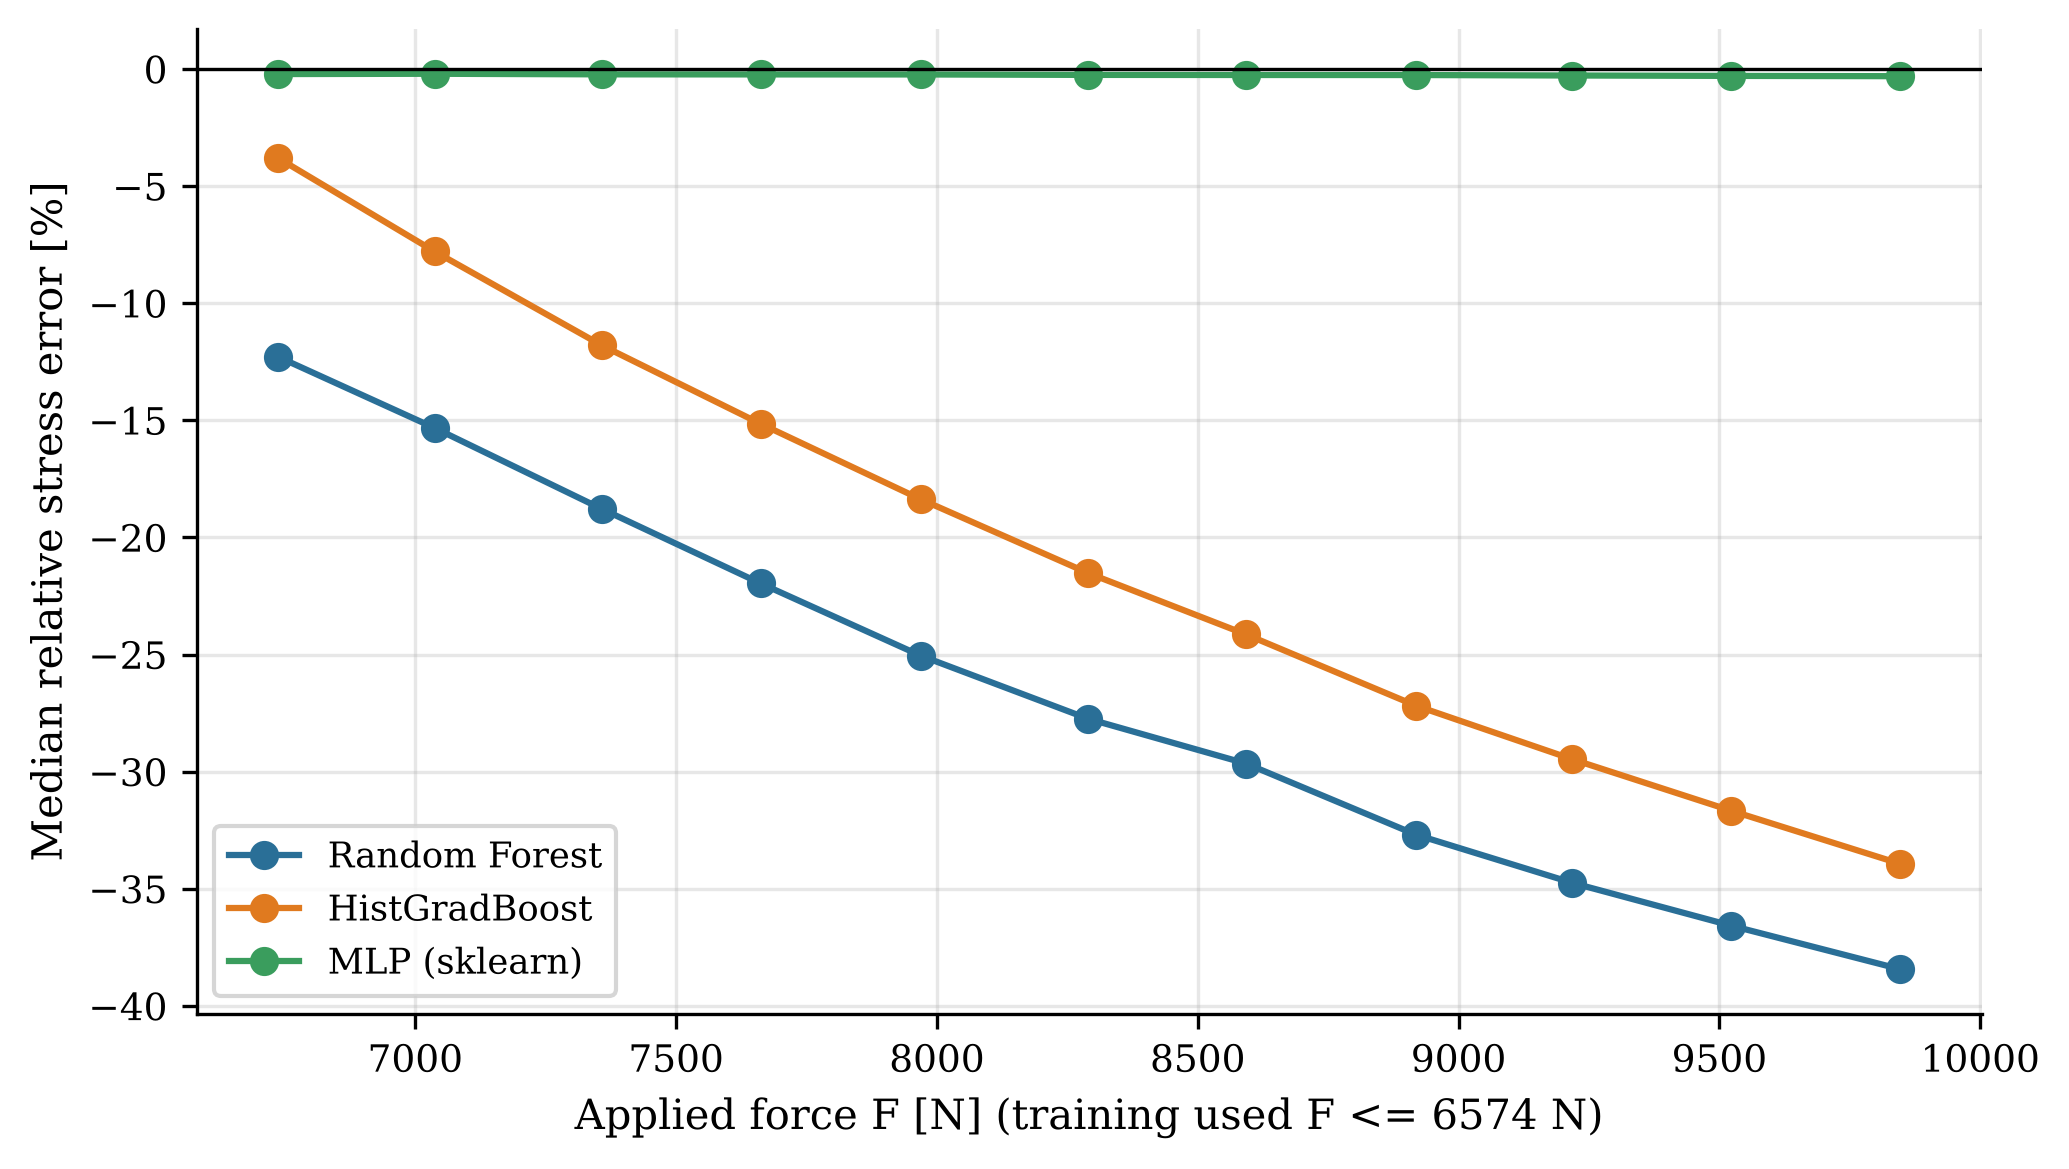
\includegraphics[width=0.62\textwidth]{15_extrapolation_force.png}
\caption{Median relative stress error versus applied force in the extrapolation test. Tree ensembles underpredict
increasingly as $F$ moves beyond the training range.}
\label{fig:ood}
\end{figure}

\subsection{Computational cost}\label{sec:timing}
Predicting the <<NTEST>> test beams took <<T_AN>>\,ms with the vectorised analytical solver, versus <<T_MLP>>\,ms (MLP),
<<T_RF>>\,ms (random forest) and <<T_GB>>\,ms (gradient boosting) on the same machine. As expected, a surrogate is
\emph{slower} than the closed-form expression it imitates; the timing is reported to avoid any implied speed-up claim.

%==================================================================== RESULTS & DISCUSSION
\section{Results and discussion}
\paragraph{Ranking.} For every regression target the MLP is the best learned model by a wide margin: its median error is
roughly <<RATIO_GB>> times smaller than gradient boosting and <<RATIO_RF>> times smaller than the random forest for stress
(Table~\ref{tab:reg}). Gradient boosting is consistently better than the random forest, which is the weakest model on
every metric.

\paragraph{Why the MLP wins.} In log space the target is a linear function of the log inputs. An MLP fed
log-standardised inputs only has to learn a nearly linear map, which it does to within
$\sim$0.1\,\%. The ablation confirms that the representation, not only the architecture, matters: the same MLP on raw
standardised inputs has a median stress error of <<RAW_S_MED>>\,\%, about <<RATIO_RAW>> times larger, because it must
synthesise products and inverse powers such as $1/h^2$ from additive units.

\paragraph{Why tree ensembles struggle.} Trees~\cite{hastie2009} approximate a function by axis-aligned, piecewise-constant pieces. A
smooth multiplicative function of six variables needs very many such pieces, and each leaf averages training targets,
which biases predictions towards the mean at the edges of the data. This is visible as heteroscedastic residuals that
grow at the extremes of the target range (Figure~\ref{fig:resid}) and as a maximum stress error of <<RF_S_MAX>>\,\% for the
random forest. Boosting reduces the bias by fitting residuals sequentially~\cite{friedman2001}, explaining its better scores.
The random forest is also hampered by averaging fully grown trees on only <<NTRAIN>> samples in a six-dimensional space.

\paragraph{Classification.} Direct classifiers must learn the curved yield boundary $\sigma_y b h^2=6FL$ from labels
alone, and their errors are concentrated close to it. Deriving the label from an accurate stress regressor is more
effective: the MLP-derived classifier made a single error out of <<NTEST>> (at true FoS $=$ <<DER_ERR_FOS>>), while
the best direct classifier (MLP) made <<MLP_C_ERR>>. Figure~\ref{fig:fosmis} shows that misclassification happens only in
a narrow band around FoS $=1$, where a small relative error in stress flips the label. For safety-related use, a
conservative margin (e.g.\ flagging $\widehat{\mathrm{FoS}}<1+k\cdot$ expected error) would be required; recall
(missed yield cases) is the more critical error.

\paragraph{Extrapolation.} When the test forces exceed the training range, tree ensembles cannot predict stresses above
the largest training targets in the corresponding leaves, so the random forest's stress $R^2$ drops to <<OOD_RF_R2>>
(Table~\ref{tab:ood}). The log-input MLP stays accurate because the learned near-linear log map continues smoothly.
This is the most practically relevant difference between the families: test-set accuracy inside the training
distribution does not guarantee sensible behaviour outside it.

%==================================================================== SENSITIVITY
\section{Sensitivity analysis}\label{sec:sens}
\subsection{One-at-a-time sweeps}
Following standard practice~\cite{saltelli2008}, each input was swept across its full range with the others fixed at the baseline (Figure~\ref{fig:sweeps}). Parts of a
sweep that violate the validity constraints (grey) lie outside the training data. The local log--log slope of each model's
prediction over the valid part of each sweep was compared with the exact exponent (Table~\ref{tab:slopes},
Figure~\ref{fig:elast}).

\begin{figure}[H]\centering
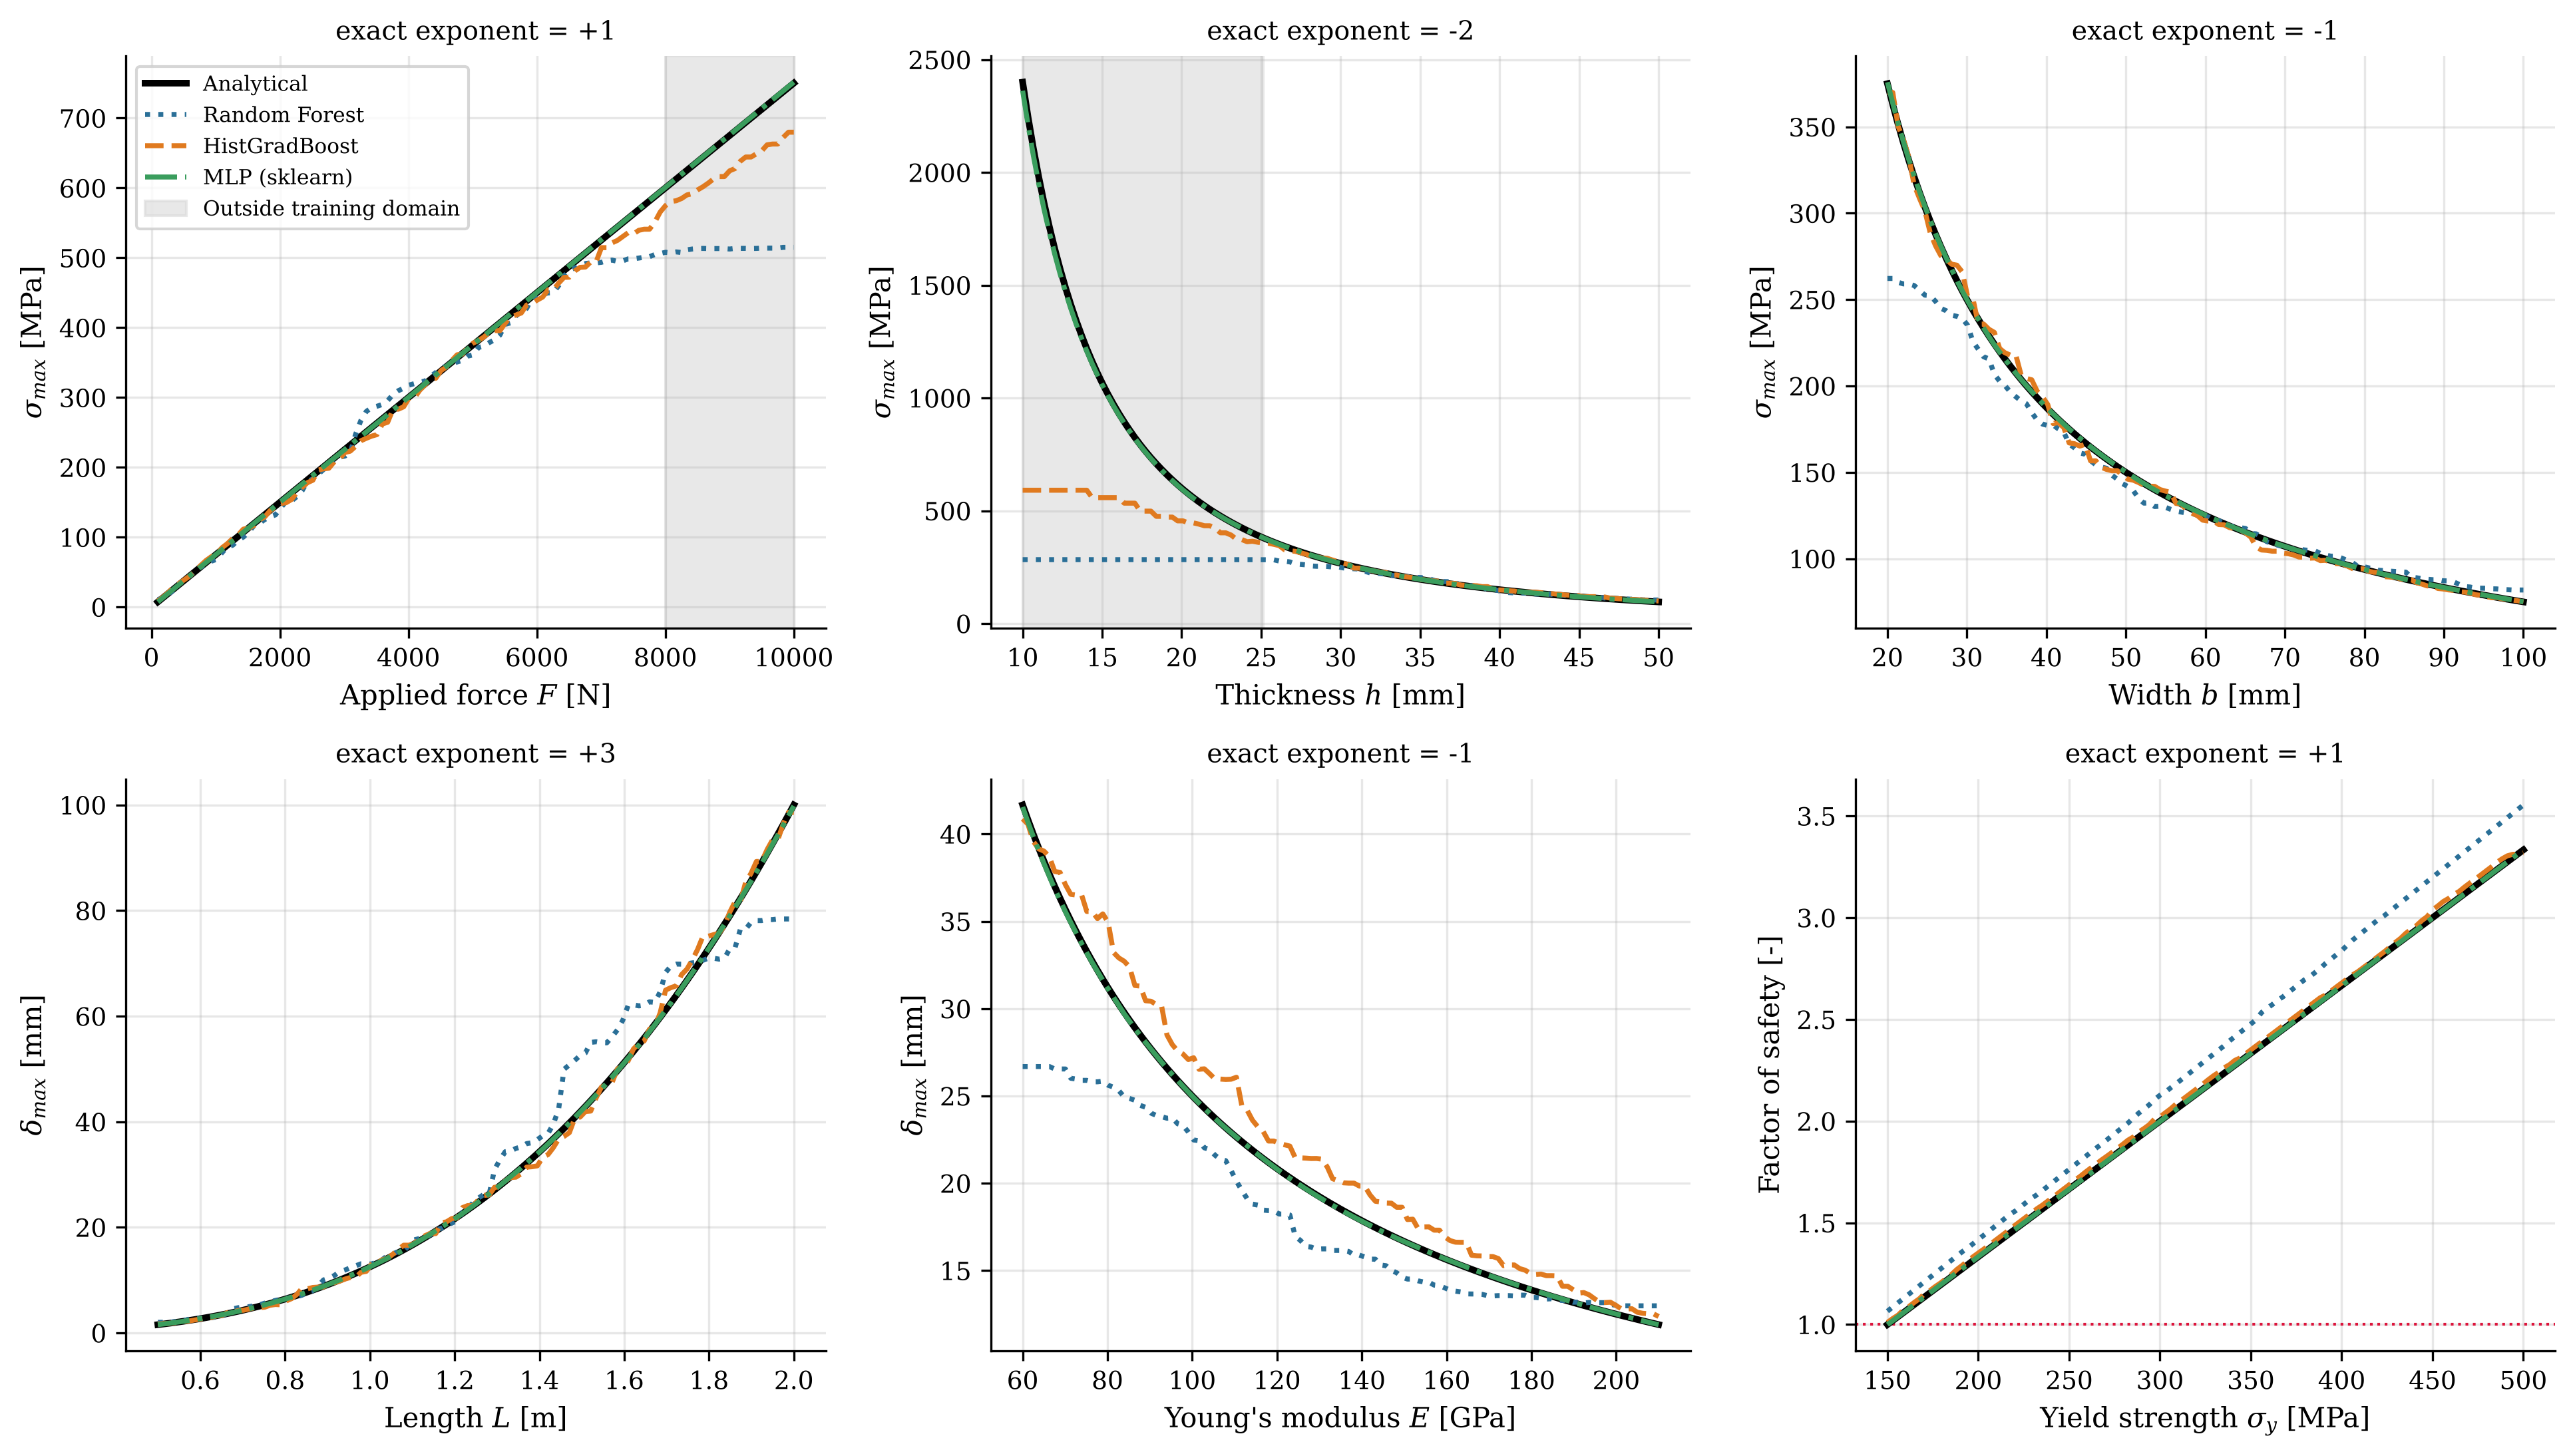
\includegraphics[width=\textwidth]{16_sensitivity_sweeps.png}
\caption{One-at-a-time sweeps around the baseline beam. Black: analytical; coloured: ML models. Grey: outside the
training domain.}
\label{fig:sweeps}
\end{figure}

\begin{table}[H]\centering\small
\caption{Elasticities $\partial\ln y/\partial\ln x$ recovered from the sweeps (valid domain only) and fraction of sweep
steps with the physically correct sign of change.}
\label{tab:slopes}
\begin{tabular}{lcrrrr}
\toprule
Effect & Exact & Random forest & Boosting & MLP & Correct-sign steps (RF / GB / MLP)\\
\midrule
<<TABLE_SLOPES>>
\bottomrule
\end{tabular}
\end{table}

\begin{figure}[H]\centering
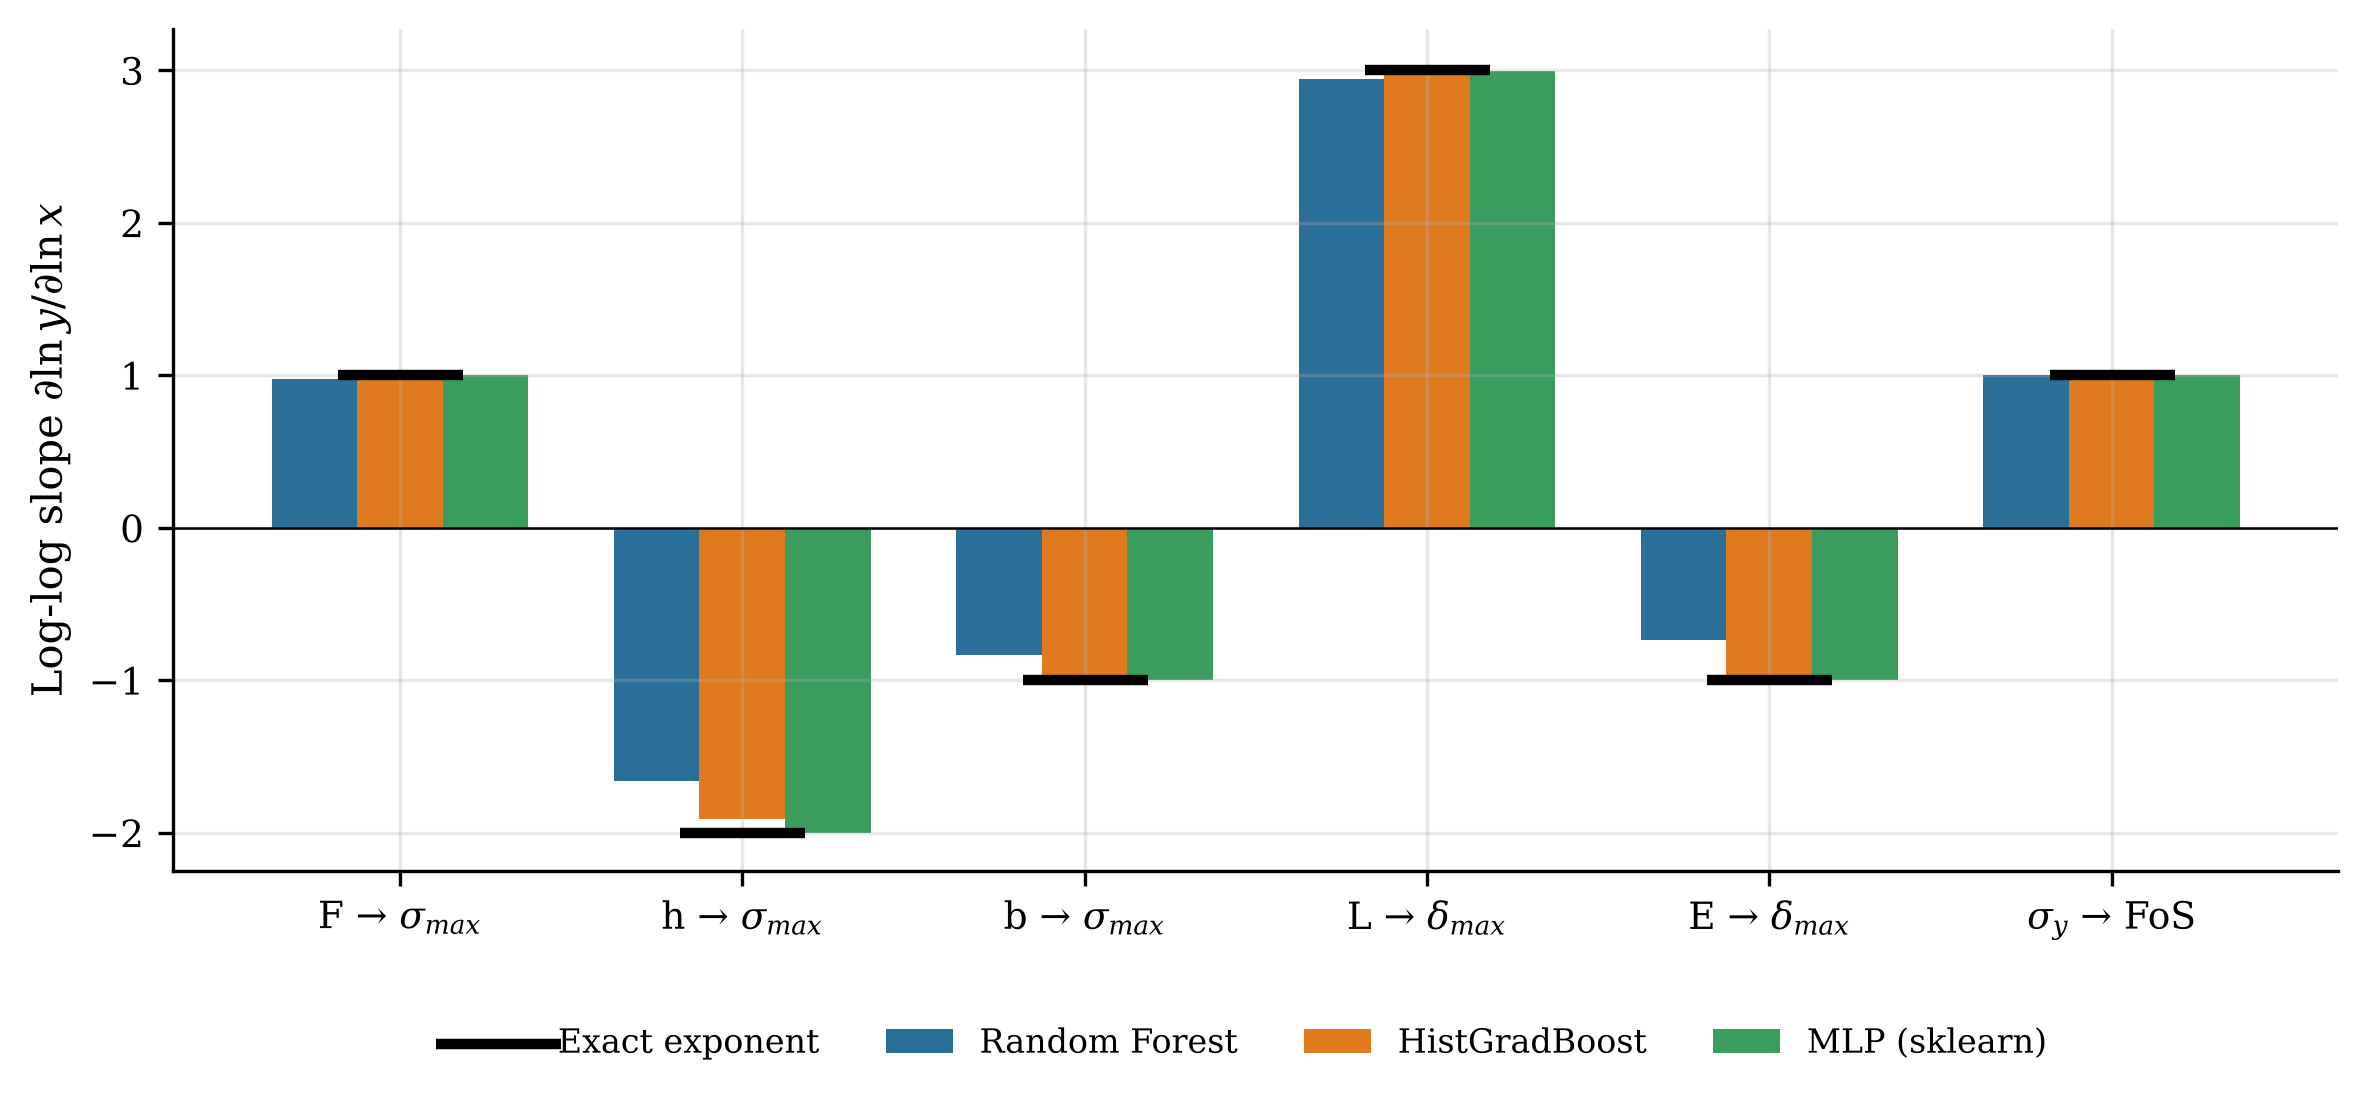
\includegraphics[width=0.78\textwidth]{17_elasticity_comparison.png}
\caption{Elasticities recovered by each model compared with the exact exponents.}
\label{fig:elast}
\end{figure}

\subsection{Physical interpretation}
\begin{itemize}
\item \textbf{Force $\to$ stress (exponent $+1$).} Stress is proportional to load; doubling $F$ doubles $\smax$. All
models capture this inside the domain; beyond the training range the tree models flatten (Figure~\ref{fig:sweeps}, top left).
\item \textbf{Thickness $\to$ stress ($-2$).} The section modulus $bh^2/6$ grows with $h^2$, so thickness is the most
efficient way to reduce stress: a 25\,\% thicker beam lowers stress by 36\,\%. Trees recover a slope of only
<<RF_H_SLOPE>> (random forest) because thin beams are rare in the filtered data.
\item \textbf{Width $\to$ stress ($-1$).} Width enters linearly in $I$ and in the section modulus, hence the weaker effect.
\item \textbf{Length $\to$ deflection ($+3$).} The cubic dependence makes span the dominant driver of deflection; doubling $L$
increases $\dmax$ eightfold.
\item \textbf{Young's modulus $\to$ deflection ($-1$).} Stiffer material reduces deflection proportionally but, for this
statically determinate beam, leaves the stress unchanged. The random forest's slope of <<RF_E_SLOPE>> shows it partly
confuses the role of $E$, which carries little variance in the data.
\item \textbf{Yield strength $\to$ FoS ($+1$).} Since $\sigma_y$ does not affect stress, FoS scales linearly with it; the
yield boundary in Figure~\ref{fig:fosmap} follows $h_{\mathrm{crit}}=\sqrt{6FL/(b\sigma_y)}$.
\end{itemize}

\subsection{Global sensitivity over the dataset}
Because $\log y=\sum_i a_i\log x_i+c$ exactly, the variance of $\log y$ can be split into contributions
$S_i=a_i\,\mathrm{Cov}(\log x_i,\log y)/\mathrm{Var}(\log y)$, which sum to one even for correlated
inputs~\cite{li2010}. Over the dataset, force accounts for <<VS_F_S>>\,\% of the log-variance of stress, while thickness
contributes only <<VS_H_S>>\,\% despite its exponent of $-2$ (Figure~\ref{fig:vs}). This is a property of the
\emph{filtered dataset}, not of beam theory: thickness varies over a narrow log-range after filtering and is
positively correlated with force, so thick beams tend to carry large loads and the two effects partly cancel.
For deflection, length (<<VS_L_D>>\,\%) and force (<<VS_F_D>>\,\%) dominate.
\begin{figure}[H]\centering
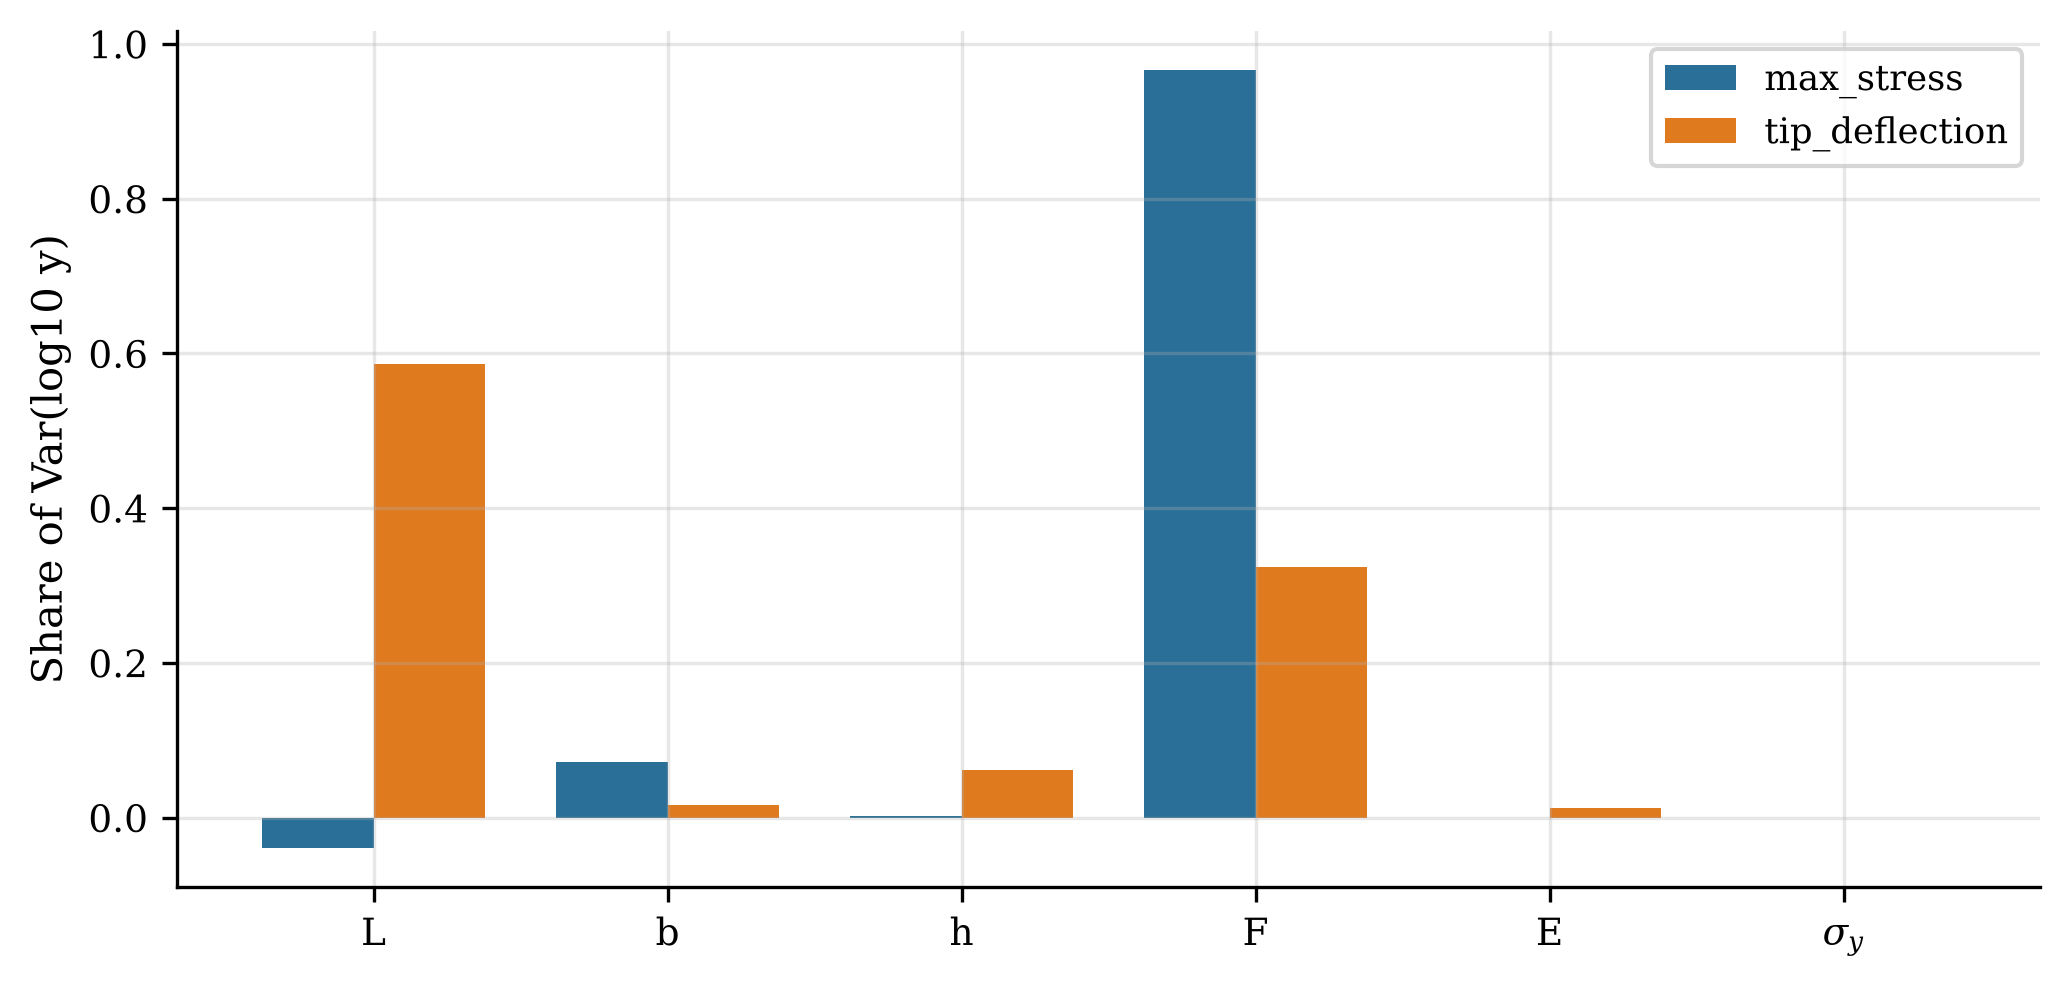
\includegraphics[width=0.62\textwidth]{18_global_variance_shares.png}
\caption{Covariance-based shares of $\mathrm{Var}(\log_{10}y)$ by input over the dataset.}
\label{fig:vs}
\end{figure}

%==================================================================== ENGINEERING INTERPRETATION
\section{Engineering interpretation}
\begin{figure}[H]\centering
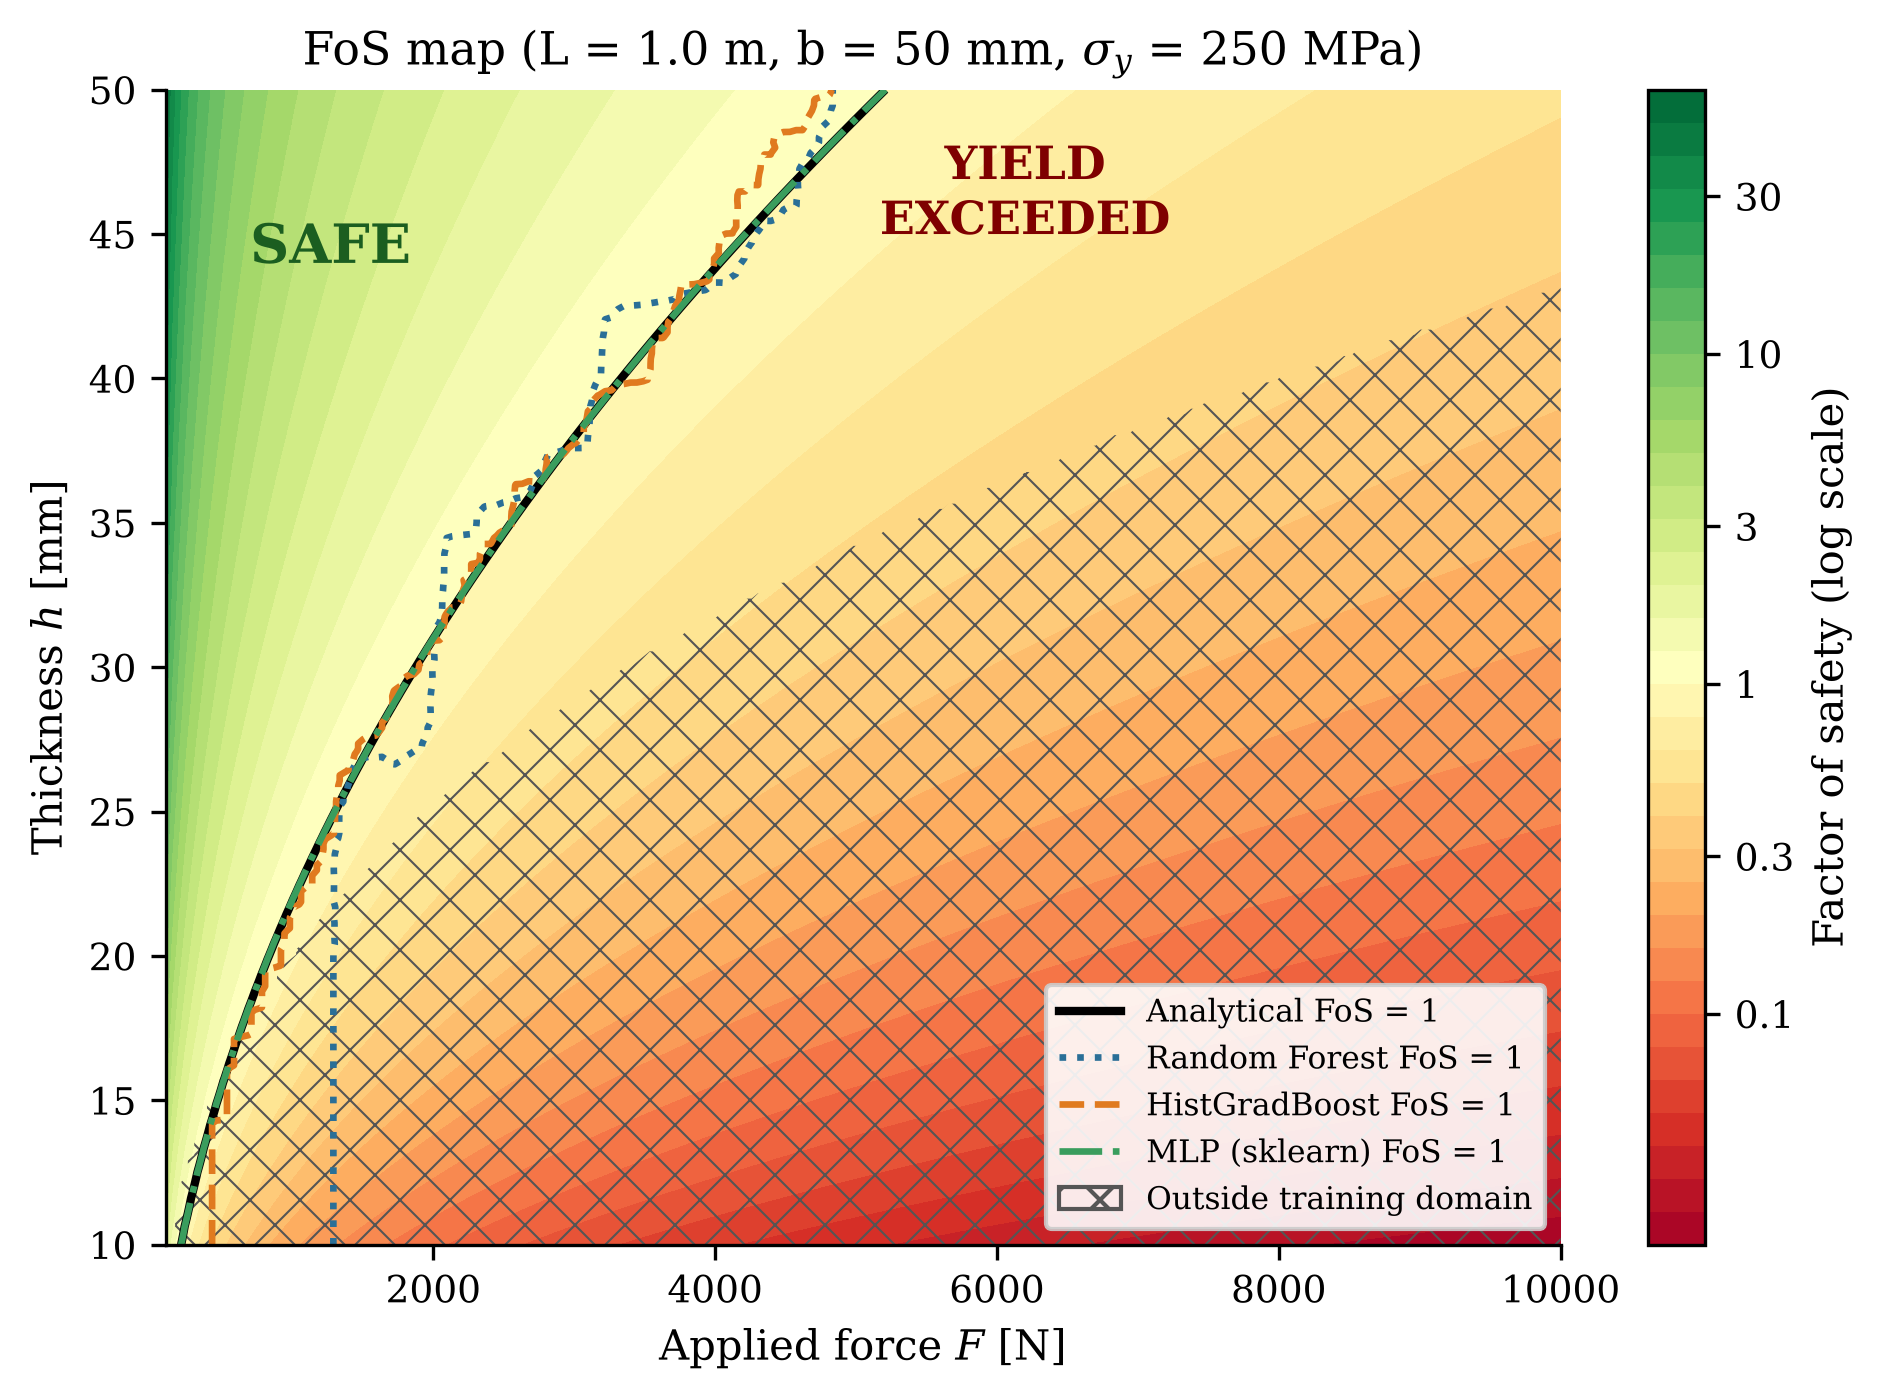
\includegraphics[width=0.75\textwidth]{08_fos_safety_map.png}
\caption{Factor-of-safety map over force and thickness (other parameters at baseline). Black: analytical yield
boundary; coloured: boundaries implied by each ML stress model. Hatched: outside the training domain.}
\label{fig:fosmap}
\end{figure}
Figure~\ref{fig:fosmap} translates the accuracy figures into design terms. The MLP boundary is indistinguishable from the
analytical curve, while the random-forest boundary is a staircase and, where it enters the hatched region, extends
vertically instead of following the curve---a direct visual consequence of piecewise-constant extrapolation. A designer
using the random forest near $h\approx 25$--35\,mm could misjudge the required thickness by a few millimetres. The
practical lessons are:
\begin{enumerate}
\item encode known physics in the representation (log transforms, dimensionless groups) where possible;
\item test learned models for physically correct trends and behaviour at and beyond the data boundary, not only for
average test error;
\item treat classifications near FoS $=1$ with an explicit safety margin, and prefer conservative errors.
\end{enumerate}

%==================================================================== LIMITATIONS
\section{Limitations}
\begin{itemize}
\item \textbf{Synthetic, noise-free data.} Targets come from a closed-form solution with no measurement noise, modelling
error or material scatter. Real experimental or FEA data would be noisier and much scarcer.
\item \textbf{Simplified mechanics.} Linear-elastic Euler--Bernoulli theory with a nominal yield check; no shear
deformation, stress concentration at the clamp, plasticity, buckling, fatigue or fracture. ``Failure'' means only that
the elastic stress reaches yield.
\item \textbf{Trivially identifiable target.} A log-linear regression is exact, so the benchmark measures how well generic
learners recover a known power law, not their ability to discover unknown physics.
\item \textbf{Sampling choices.} Uniform sampling with rejection produces non-uniform, correlated inputs; independent
$(E,\sigma_y)$ sampling does not reflect real alloy pairings. Results depend on these choices.
\item \textbf{Software backends.} <<BACKEND_LIMIT>>
\item \textbf{Limited tuning.} Small hyper-parameter grids were used; tree models might improve with larger ensembles,
but cannot overcome their extrapolation behaviour.
\end{itemize}

%==================================================================== FUTURE SCOPE
\section{Future scope}
\begin{itemize}
\item Replace the analytical solver with FEA (e.g.\ 2-D plane-stress or 3-D solid models) to include stress concentrations
at the support, and study accuracy versus number of expensive simulations (learning curves, active learning).
\item Extend to load cases and geometries without closed-form solutions: distributed loads, I-sections, plates with holes.
\item Predict full stress or displacement fields with convolutional or graph neural networks instead of scalar maxima.
\item Physics-informed training (dimensionless inputs, monotonicity constraints, PINN-style residual losses).
\item Add material nonlinearity (elasto-plastic response) and noisy labels; quantify predictive uncertainty
(ensembles, quantile regression) to set rational classification margins.
\end{itemize}

%==================================================================== REFERENCES
\begin{thebibliography}{99}\small
\bibitem{gere2013} J.~M. Gere and B.~J. Goodno, \emph{Mechanics of Materials}, 8th ed. Stamford, CT: Cengage Learning, 2013.
\bibitem{budynas2015} R.~G. Budynas and J.~K. Nisbett, \emph{Shigley's Mechanical Engineering Design}, 10th ed. New York: McGraw-Hill, 2015.
\bibitem{forrester2008} A.~I.~J. Forrester, A. S\'obester and A.~J. Keane, \emph{Engineering Design via Surrogate Modelling: A Practical Guide}. Chichester: Wiley, 2008.
\bibitem{breiman2001} L. Breiman, ``Random forests,'' \emph{Machine Learning}, vol.~45, no.~1, pp.~5--32, 2001.
\bibitem{friedman2001} J.~H. Friedman, ``Greedy function approximation: A gradient boosting machine,'' \emph{Annals of Statistics}, vol.~29, no.~5, pp.~1189--1232, 2001.
\bibitem{chen2016} T. Chen and C. Guestrin, ``XGBoost: A scalable tree boosting system,'' in \emph{Proc.\ 22nd ACM SIGKDD Int.\ Conf.\ Knowledge Discovery and Data Mining}, 2016, pp.~785--794.
\bibitem{ke2017} G. Ke \emph{et al.}, ``LightGBM: A highly efficient gradient boosting decision tree,'' in \emph{Advances in Neural Information Processing Systems 30}, 2017.
\bibitem{hornik1989} K. Hornik, M. Stinchcombe and H. White, ``Multilayer feedforward networks are universal approximators,'' \emph{Neural Networks}, vol.~2, no.~5, pp.~359--366, 1989.
\bibitem{kingma2015} D.~P. Kingma and J. Ba, ``Adam: A method for stochastic optimization,'' in \emph{Proc.\ 3rd Int.\ Conf.\ Learning Representations (ICLR)}, 2015.
\bibitem{paszke2019} A. Paszke \emph{et al.}, ``PyTorch: An imperative style, high-performance deep learning library,'' in \emph{Advances in Neural Information Processing Systems 32}, 2019.
\bibitem{pedregosa2011} F. Pedregosa \emph{et al.}, ``Scikit-learn: Machine learning in Python,'' \emph{Journal of Machine Learning Research}, vol.~12, pp.~2825--2830, 2011.
\bibitem{hastie2009} T. Hastie, R. Tibshirani and J. Friedman, \emph{The Elements of Statistical Learning}, 2nd ed. New York: Springer, 2009.
\bibitem{saltelli2008} A. Saltelli \emph{et al.}, \emph{Global Sensitivity Analysis: The Primer}. Chichester: Wiley, 2008.
\bibitem{li2010} G. Li, H. Rabitz, P.~E. Yelvington, O.~O. Oluwole, F. Bacon, C.~E. Kolb and J. Schoendorf, ``Global sensitivity analysis for systems with independent and/or correlated inputs,'' \emph{Journal of Physical Chemistry A}, vol.~114, no.~19, pp.~6022--6032, 2010.
\bibitem{harris2020} C.~R. Harris \emph{et al.}, ``Array programming with NumPy,'' \emph{Nature}, vol.~585, pp.~357--362, 2020.
\bibitem{hunter2007} J.~D. Hunter, ``Matplotlib: A 2D graphics environment,'' \emph{Computing in Science \& Engineering}, vol.~9, no.~3, pp.~90--95, 2007.
\end{thebibliography}

\appendix
\section{Reproducing the results}
\begin{verbatim}
pip install -r requirements.txt
python run_pipeline.py           # full pipeline + tests
python run_pipeline.py --report  # also rebuild this PDF
streamlit run app.py             # dashboard
\end{verbatim}
All numbers in this report are inserted automatically from \texttt{results/experiment\_results.json},
\texttt{results/sensitivity\_results.json}, \texttt{models/*/config.json} and \texttt{data/generation\_stats.json} by
\texttt{report/build\_report.py}.
\end{document}
